%%%%%%%% ICML 2022 EXAMPLE LATEX SUBMISSION FILE %%%%%%%%%%%%%%%%%
\pdfoutput=1

\documentclass{article}

% Recommended, but optional, packages for figures and better typesetting:
\usepackage{microtype}
\usepackage{graphicx}
\usepackage{subfigure}
\usepackage{booktabs} % for professional tables
\usepackage{xspace}
\usepackage{makecell}
\usepackage{diagbox}
\usepackage{nicefrac}
\usepackage{amsmath}
\usepackage{float}
% \usepackage{minted}
\newcommand{\pushright}[1]{\ifmeasuring@#1\else\omit\hfill$\displaystyle#1$\fi\ignorespaces}

% \setminted{fontsize=\small}
\usepackage{listings}
\lstset{
    language=Python,
    basicstyle=\ttfamily\small,
    keywordstyle=\color{blue},
    commentstyle=\color{green},
    stringstyle=\color{red},
    backgroundcolor=\color{gray!15},
    morekeywords={GlobalLocalTransformerDecoder, forward, prepare_input, __init__},
    showstringspaces=false,
    breaklines=true,
}
\newcommand{\fastslow}[0]{\textsc{MegaByte}\xspace}
\newcommand{\megabyte}[0]{\fastslow}
\newcommand{\bpb}[0]{bpb\xspace}
\newcommand{\h}[1]{h^\text{#1}}%_{#2}}
\newcommand{\inR}[1]{\in\mathbb{R}^{#1}}
\newcommand{\transformer}[2]{\text{transformer}^{\text{#1}}(#2)}
\newcommand{\Lglobal}[0]{L_{\text{global}}}
\newcommand{\Llocal}[0]{L_{\text{local}}}

\newcommand{\todo}[1]{\textcolor{red}{[TODO: #1]}}
\newcommand{\wip}[1]{\textcolor{purple}{#1}}
\newcommand{\mike}[1]{\textcolor{blue}{[Mike: #1]}}
\newcommand{\lly}[1]{\textcolor{magenta}{[LL: #1]}}



% hyperref makes hyperlinks in the resulting PDF.
% If your build breaks (sometimes temporarily if a hyperlink spans a page)
% please comment out the following usepackage line and replace
% \usepackage{icml2022} with \usepackage[nohyperref]{icml2022} above.
\usepackage{hyperref}


% Attempt to make hyperref and algorithmic work together better:
\newcommand{\theHalgorithm}{\arabic{algorithm}}

% Use the following line for the initial blind version submitted for review:
\usepackage[accepted]{icml2022}

% If accepted, instead use the following line for the camera-ready submission:
% \usepackage[accepted]{icml2022}

% For theorems and such
\usepackage{amsmath}
\usepackage{amssymb}
\usepackage{mathtools}
\usepackage{amsthm}

% if you use cleveref..
\usepackage[capitalize,noabbrev]{cleveref}

%%%%%%%%%%%%%%%%%%%%%%%%%%%%%%%%
% THEOREMS
%%%%%%%%%%%%%%%%%%%%%%%%%%%%%%%%
\theoremstyle{plain}
\newtheorem{theorem}{Theorem}[section]
\newtheorem{proposition}[theorem]{Proposition}
\newtheorem{lemma}[theorem]{Lemma}
\newtheorem{corollary}[theorem]{Corollary}
\theoremstyle{definition}
\newtheorem{definition}[theorem]{Definition}
\newtheorem{assumption}[theorem]{Assumption}
\theoremstyle{remark}
\newtheorem{remark}[theorem]{Remark}

% Todonotes is useful during development; simply uncomment the next line
%    and comment out the line below the next line to turn off comments
%\usepackage[disable,textsize=tiny]{todonotes}
% \usepackage[textsize=tiny]{todonotes}


% The \icmltitle you define below is probably too long as a header.
% Therefore, a short form for the running title is supplied here:
%\icmltitlerunning{Bytes In, Bytes Out: Efficient Byte-level Modeling with Multiscale Transformers}

\begin{document}

\twocolumn[
\icmltitle{\fastslow: Predicting Million-byte Sequences with Multiscale Transformers}

% It is OKAY to include author information, even for blind
% submissions: the style file will automatically remove it for you
% unless you've provided the [accepted] option to the icml2022
% package.

% List of affiliations: The first argument should be a (short)
% identifier you will use later to specify author affiliations
% Academic affiliations should list Department, University, City, Region, Country
% Industry affiliations should list Company, City, Region, Country

% You can specify symbols, otherwise they are numbered in order.
% Ideally, you should not use this facility. Affiliations will be numbered
% in order of appearance and this is the preferred way.
\icmlsetsymbol{equal}{*}

\begin{icmlauthorlist}
\icmlauthor{Lili Yu}{equal,meta}
\icmlauthor{Dániel Simig}{equal,meta}
\icmlauthor{Colin Flaherty}{equal,augment}
\icmlauthor{Armen Aghajanyan}{meta}
\icmlauthor{Luke Zettlemoyer}{meta}
\icmlauthor{Mike Lewis}{meta}

%\icmlauthor{Firstname3 Lastname3}{comp}
%\icmlauthor{Firstname4 Lastname4}{sch}
%\icmlauthor{Firstname5 Lastname5}{yyy}
%\icmlauthor{Firstname6 Lastname6}{sch,yyy,comp}
%\icmlauthor{Firstname7 Lastname7}{comp}
%\icmlauthor{}{sch}
%\icmlauthor{Firstname8 Lastname8}{sch}
%\icmlauthor{Firstname8 Lastname8}{yyy,comp}
%\icmlauthor{}{sch}
%\icmlauthor{}{sch}
\end{icmlauthorlist}

\icmlaffiliation{augment}{Augment Computing. Work performed while at Meta AI.}
\icmlaffiliation{meta}{Meta AI.}
%\icmlaffiliation{yyy}{Department of XXX, University of YYY, Location, Country}
%\icmlaffiliation{comp}{Company Name, Location, Country}
%\icmlaffiliation{sch}{School of ZZZ, Institute of WWW, Location, Country}

\icmlcorrespondingauthor{Lili Yu}{liliyu@meta.com}
% \icmlcorrespondingauthor{Daniel Simig}{simigd@gmail.com}
% \icmlcorrespondingauthor{Colin Flaherty}{colin@augmentcode.com}
\icmlcorrespondingauthor{Mike Lewis}{mikelewis@meta.com}


% You may provide any keywords that you
% find helpful for describing your paper; these are used to populate
% the "keywords" metadata in the PDF but will not be shown in the document
\icmlkeywords{Machine Learning, ICML}

\vskip 0.3in
]

% this must go after the closing bracket ] following \twocolumn[ ...

% This command actually creates the footnote in the first column
% listing the affiliations and the copyright notice.
% The command takes one argument, which is text to display at the start of the footnote.
% The \icmlEqualContribution command is standard text for equal contribution.
% Remove it (just {}) if you do not need this facility.

%\printAffiliationsAndNotice{}  % leave blank if no need to mention equal contribution
\printAffiliationsAndNotice{\icmlEqualContribution} % otherwise use the standard text.

\begin{abstract}
Autoregressive transformers are spectacular models for short sequences but scale poorly to long sequences such as high-resolution images, podcasts, code, or books. We propose \fastslow, a multi-scale decoder architecture that enables end-to-end differentiable modeling of sequences of over one million bytes.
\fastslow segments sequences into patches and uses a \emph{local} submodel within patches and a \emph{global} model between patches. This enables sub-quadratic self-attention, much larger feedforward layers for the same compute, and improved parallelism during decoding---unlocking  better performance at reduced cost for both training and generation. 
Extensive experiments show that \fastslow allows byte-level models to perform competitively with subword models on long context language modeling, achieve state-of-the-art density estimation on ImageNet, and model audio from raw files. Together, these results establish the  viability of tokenization-free autoregressive sequence modeling at scale. 
\end{abstract}

\section{Introduction}
\label{sec:intro}
Sequences of millions of bytes are ubiquitous; for example, music, image, or video files typically consist of multiple megabytes. 
However, large transformer decoders (LLMs) typically only use several thousand tokens of context \citep{gpt3,Zhang2022OPT:Models}---both because of the quadratic cost of self-attention but also, more importantly, the cost of large feedforward networks per-position. 
This severely limits the set of tasks where LLMs can be applied.

\begin{figure}
    \centering
    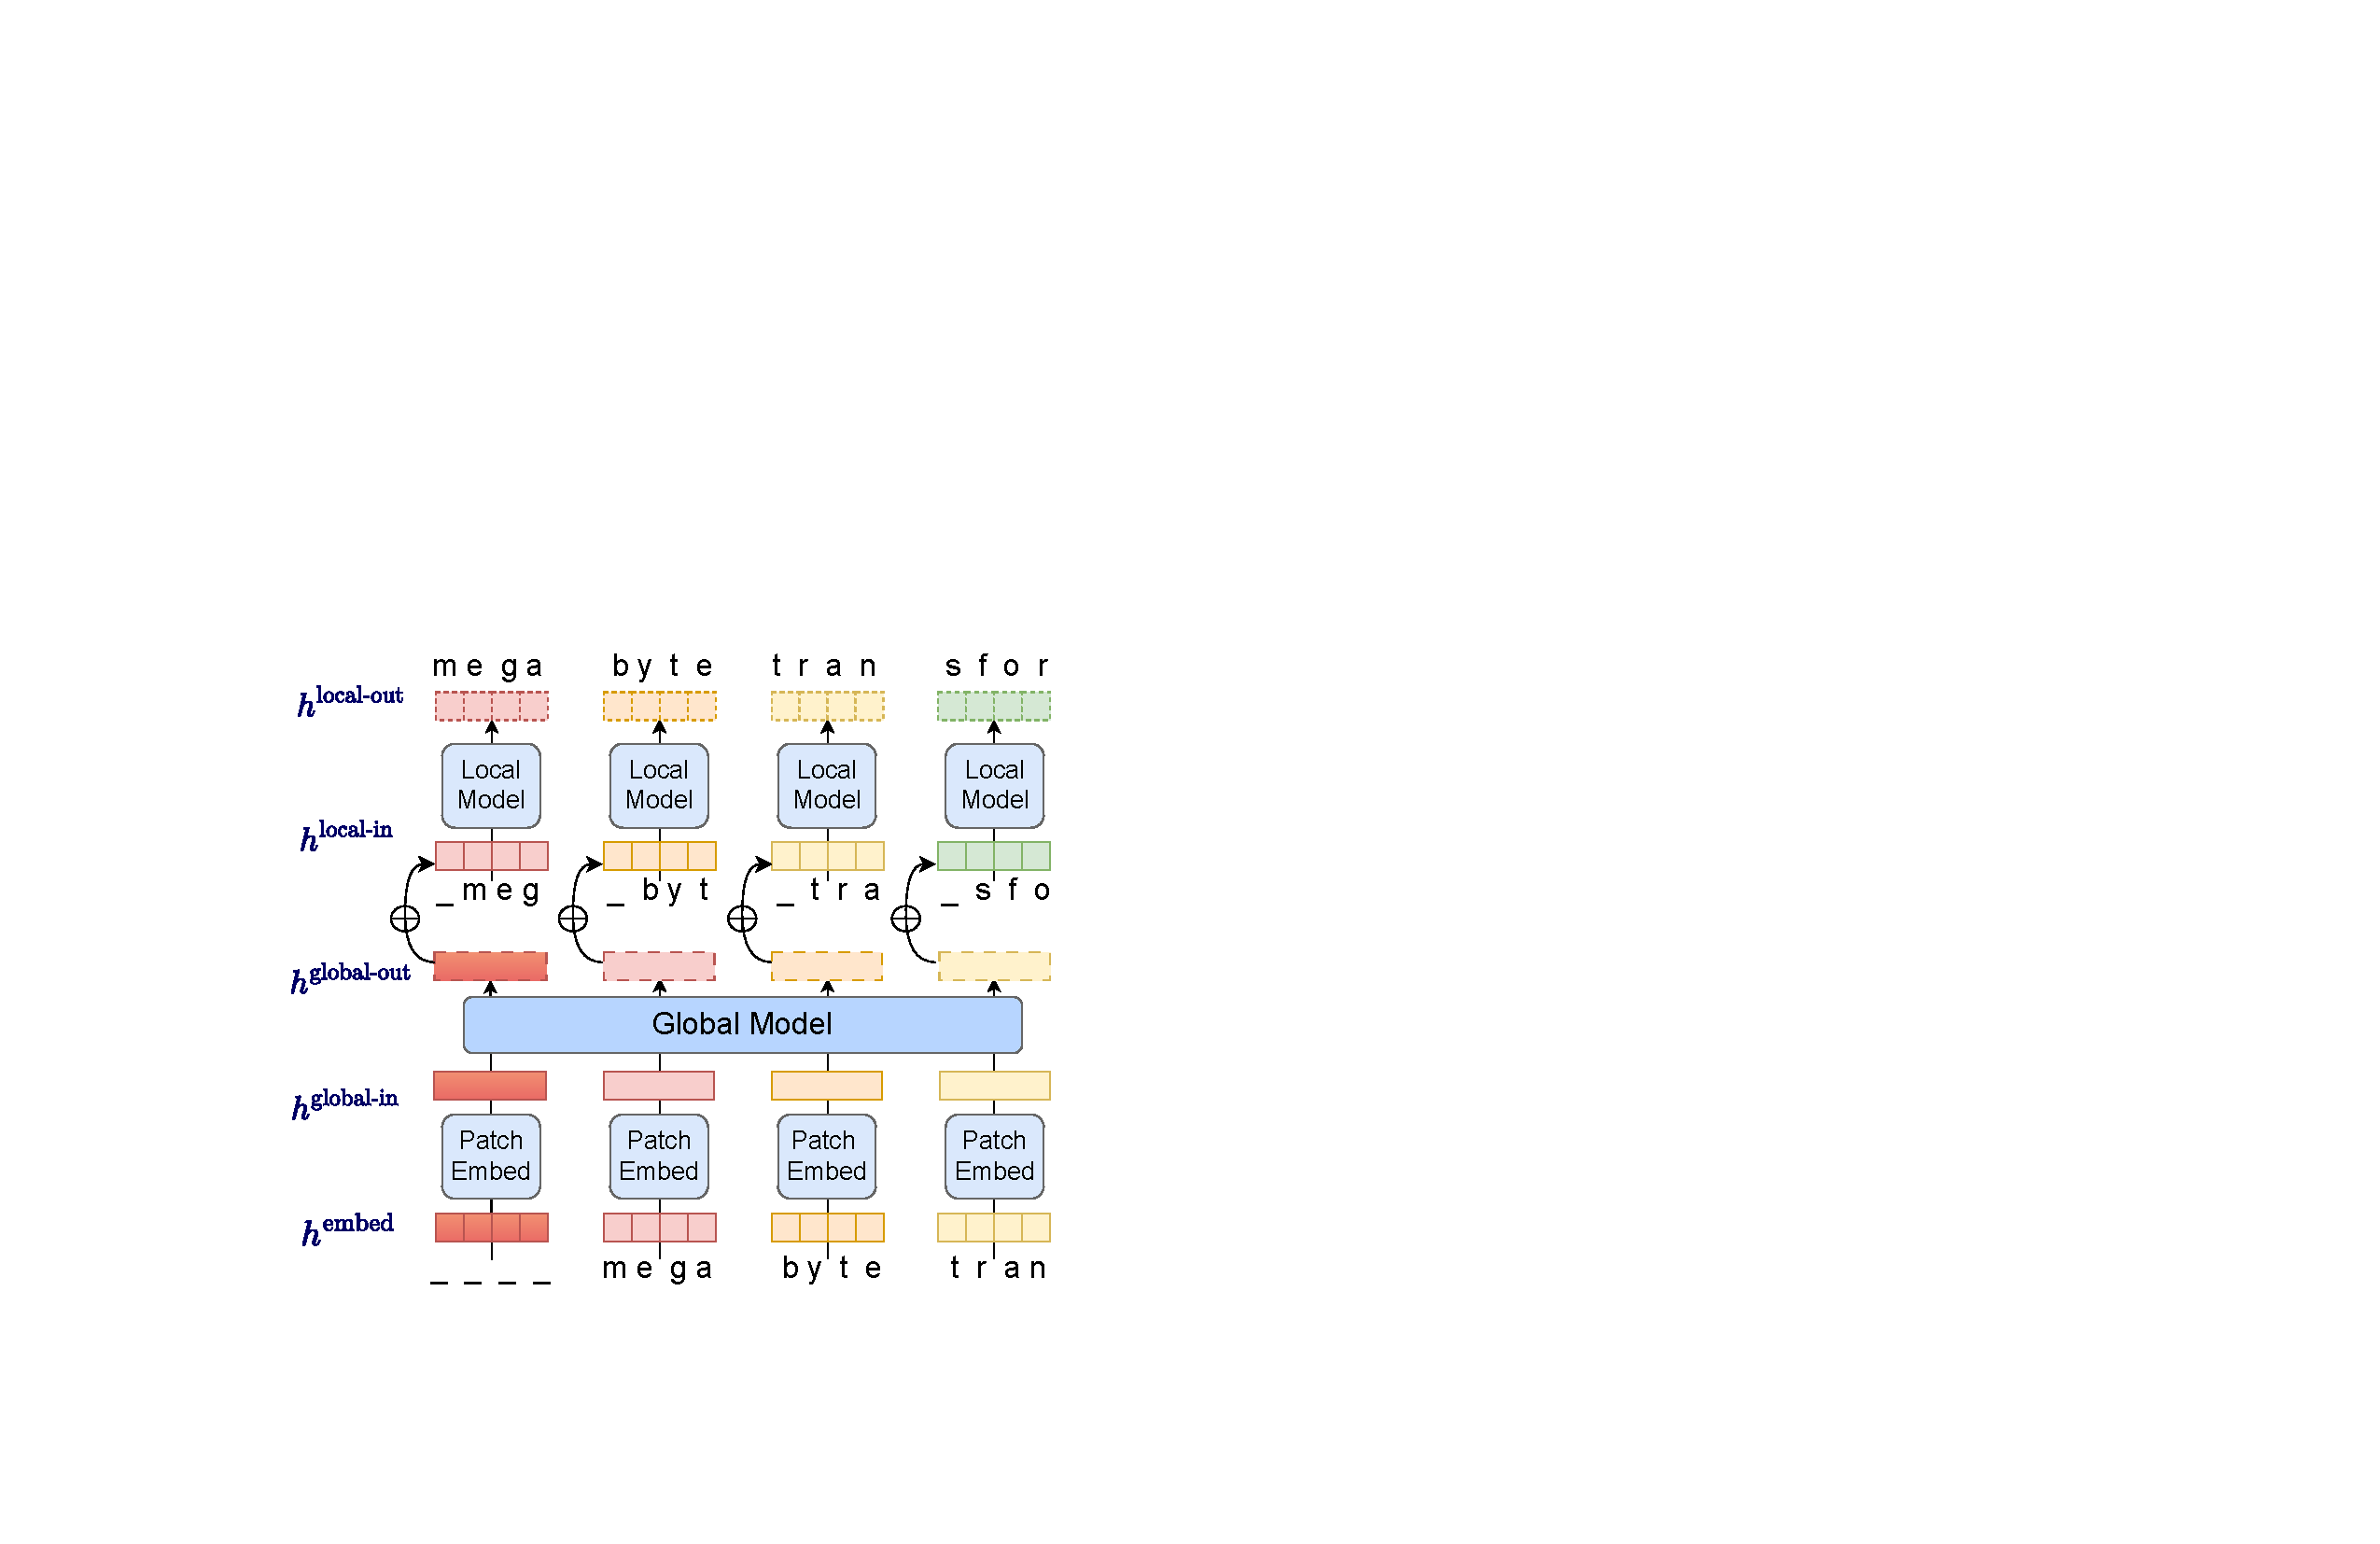
\includegraphics[width=\linewidth]{figs/fastslow3.pdf}
    % \caption{Illustration of \megabyte model architecture and the modeling of "megabyte transformer" byte sequence. In this figure, padding is represented by underscores ("_"), spaces are represented by quotes ("' '"), and the addition operator is represented by a plus sign.}
    \vspace*{-5mm}
     \caption{Overview of \megabyte with patch size $P=4$. 
     A small \emph{local} model autoregressively predicts each patch byte-by-byte, using the output of a larger \emph{global} model to condition on previous patches.
     %A large \emph{global} model performs self-attention over previous patches, and a smaller \emph{local} model autoregressively predicts each patch byte-by-byte. 
     Global and Local inputs are padded by $P$ and $1$ token respectively to avoid leaking information about future tokens.
     %Initial patch embeddings are made by concatenating byte embeddings.
     %The \emph{global} model enriches patch embeddings by performing self-attention over previous patches.
     %We then add byte embeddings (padded by 1), and an instance of a smaller \emph{local} model autoregressively  
     %The sequences is padded by P tokens and each byte is embedded ($h^{embed}$}. Byte embeddings are 
    \label{fig:framework}
    }
\end{figure}
We introduce \fastslow, a new approach to modeling long byte sequences.
First, byte sequences are segmented into fixed-sized patches, loosely analogous to tokens.
Our model then consists of three parts: (1) a \emph{patch embedder}, which simply encodes a patch by losslessly concatenating embeddings of each byte, (2) a \emph{global} module, a large autoregressive transformer that inputs and outputs patch representations and (3) a \emph{local} module, a small autoregressive model that predicts bytes within a patch. 
Crucially, we observe that for many tasks, most byte predictions are relatively easy (for example, completing a word given the first few characters), meaning that large networks per-byte are unnecessary, and a much smaller model can be used for intra-patch modelling.

%While many approaches to modelling long sequences have focused on optimizing attention layers \citep{}, the large majority of compute in large language models is used by position-wise feedforward layers \citep{}. To reduce this cost, we must either use smaller feedforward layers (reducing performance) or compressing the sequence length (which is challenging with decoder-only models, where an output is needed at each timestep). These constraints lead to our multi-scale design, in which long range and short range decisions are handled by separate modules.

The \megabyte architecture gives three major improvements over Transformers for long sequence modelling:
\begin{enumerate}
    \item \textbf{Sub-quadratic self-attention} Most work on long sequence models has focused on mitigating the quadratic cost of self-attention. \megabyte decomposes long sequences into two shorter sequences, and optimal patch sizes reduces the self-attention cost to $O(N^{\frac{4}{3}})$, which remains tractable for even long sequences.
    \item \textbf{Per-patch feedforward layers} In GPT3-size models, more than 98\% of FLOPS are used in computing position-wise feedforward layers. \megabyte uses large feedforward layers per-patch rather than per-position, enabling much larger and more expressive models for the same cost. With patch size $P$, where a baseline transformer would use the same feedforward layer with $m$ parameters $P$ times, \megabyte can use a layer with $mP$ parameters once for the same cost.
    \item \textbf{Parallelism in Decoding} Transformers must perform all computations serially during generation because the input to each timestep is the output from the previous timestep. By generating representations for patches in parallel, \megabyte allows greater parallelism during generation. For example, a \megabyte model with 1.5B parameters can generate sequences 40\% \emph{faster} than a standard 350M Transformer, whilst also improving perplexity when trained with the same compute. %, increasing generation speed by up to \mike{XX}x.
\end{enumerate}

Together, these improvements allow us to train much larger and better-performing models for the same compute budget, scale to very long sequences, and improve generation speed during deployment.



\fastslow also provides a strong contrast to existing autoregressive models that typically use some form of tokenization, where sequences of bytes are mapped to larger discrete tokens \citep{bpe,dalle,hubert}.
%, remains the most common approach to scaling LLMs to longer sequences.
Tokenization complicates pre-processing, multi-modal modelling, and transfer to new domains, while hiding useful structure from the model. It also means that most state-of-the-art models are not truly end to end.
The most widely used approaches to tokenization require language-specific heuristics \citep{gpt2} or lose information \citep{dalle}.
Replacing tokenization with efficient and performant byte models would therefore have many advantages.

We conduct extensive experiments for both \fastslow and strong baselines. We use a fixed compute and data budget across all models 
to focus our comparisons solely on the model architecture rather than training resources, which are known to benefit all models. We find that \fastslow allows byte-level models to perform competitively with subword models on long context language modeling, achieve state-of-the-art perplexities for density estimation on ImageNet, and allow audio modelling from raw audio files. Together, these results establish the viability of tokenization-free autoregressive sequence modeling at scale.

\section{\megabyte Transformer}
\subsection{Overview}
\label{sec:fastslow}





%\subsection{Patch Encoder}
%\subsection{Slow Model}
%\subsection{Fast Model}
%\paragraph{Cross-Patch Self Attention}
%\subsection{Interface Between Slow and Fast Models}

% At a high-level, 






\begin{figure*}[t]
\begin{minipage}{0.7\linewidth}
\begin{align*}
%x^{\text{padded}} &= ([\text{PAD}]\times P) + x_{0:(T-P)}\\
\h{embed}_{t}\,\,\,\,\,\,\,\,&= E^\text{global-embed}_{x_t}+E^\text{pos}_t  & t\in [0..T), E^{\text{global-embed}}\inR{V\times D_G},\\& &E^{\text{pos}}\inR{T\times D_G}, \h{embed}\inR{T\times D_G}  \\
% \h{global-in}_{0} &= [E^{\text{pad}}_0,..,E^{\text{pad}}_{P-1}] & E^{\text{pad}}\inR{D_G}, K=\frac{T}{P}\\
% \h{global-in}_{k} &= \h{embed}_{((k-1)\cdot P):(k\cdot P)} & k\in [1,..,K) \\
\h{global-in}_{k} \,\,\,\,\,&= 
\begin{cases}
E^{\text{global-pad}}, & \text{if } k = 0, \\
\h{embed}_{((k-1)\cdot P):(k \cdot P)}, & k\in [1,..,K),  \\
\end{cases}  & E^{\text{global-pad}}\inR{P\times D_G}, K=\frac{T}{P}
\\
\h{global-out}_{0:K} \,\,\,&= \transformer{global}{\h{global-in}_{0:K}}  & \h{global-out}\inR{K\times P\cdot D_G},\h{global-in}\inR{K\times P\cdot D_G}\\
%\h{local-in}_{k,0} &= \h{global-out}_{k,0:D_G} & \h{local-in}\inR{K\times P \times D_G} \\
%\h{local-in}_{k,p} &= w^{\text{GL}}\h{global-out}_{k,(p\cdot D_G):((p+1)\cdot D_G)} + E^\text{local-embed}_{x_{(k\cdot P + p - 1)}}  &  w^{\text{GL}}\inR{D_G\times D_L}, E^{\text{local-embed}}\inR{V\times D_L}, p\in [0,..,P),   \\
\h{local-in}_{k,p} \,\,\,\,\,\,\,&= w^{\text{GL}}\h{global-out}_{k,(p\cdot D_G):((p+1)\cdot D_G)} + 
\begin{cases}
E^\text{local-pad}, & \text{if } p=0   \\
E^\text{local-embed}_{x_{(k\cdot P + p - 1)}}, & p\in [1,..,P)   \\
\end{cases} &  
\begin{array}{r}
E^{\text{local-pad}}\inR{D_L} , w^{\text{GL}}\inR{D_G\times D_L}\\ E^{\text{local-embed}}\inR{V\times D_L}
\end{array}\hspace{-2mm}
\\
\h{local-out}_{k,0:P} \,\,\,\,\,&= \transformer{local}{\h{local-in}_{k,0:P}}  & \h{local-in}_{k,p}\inR{D_L}, \h{local-out}\inR{K\times P\cdot D_L} \\
p(x_{t}|x_{0:t}) &= \text{softmax}{(E^\text{local-embed}\h{local-out}_{k,p})}_{x_t}  & t=k\cdot P+p\,
\end{align*}
\end{minipage}
\caption{Summary of \megabyte with vocabulary $V$, sequence length $T$, global and local dimensions $D_G$ and $D_L$, and $K$ patches of size $P$. Transformer layers use masked self attention to not observe information from future timesteps. 
}
\end{figure*}
% K\times P\cdot D_G
 % \h{local-in}\inR{K\times P \times D_L} 



% , while possessing many of the desirable properties of the Transformer architecture; including support for parallelism techniques enabling efficient scaling, a lack of recurrence, permutation invariance across the entire context, a single cross-entropy objective enabling end-to-end differentiation, and general architectural simplicity. 
\megabyte is an autoregressive model for efficiently modeling long input sequences. \megabyte is comprised of 3 components: (1) a \emph{patch embedder} that inputs a discrete sequence, embeds each element, and chunks it into patches of length $P$ (2) a large \emph{global} Transformer that contextualizes patch representations by performing self-attention over previous patches, and (3) a smaller \emph{local} Transformer that inputs a contextualized patch representation from the global model, and autoregressively predict the \emph{next} patch.


% Specifically, consider that any document $X$ (text, image or speech) can be serialized as a sequence of $t$ bytes $X\in \mathbb{R}^t$. These bytes can then be partitioned into small “patches” of $p$ contiguous bytes each, resulting in a compressed document encoding $\tilde{X}\in \mathbb{R}^{\nicefrac{t}{p}}$. Increasing $p$ allows us to dramatically compress the sequence length of $\tilde{X}$, which we can then efficiently model with a large language model.

%In general, any input of any modality can be represented as a sequence of $t$ bytes denoted by  $X = \{ \mathbf{x}_i \}_{i=1}^t$, where each $\mathbf{x}_i$ belongs to the set $\{ 0, 1, \dots, 255\}$. To compress $X$ for more efficient modeling, we partition the byte sequence into small, contiguous patches of length $p$, yielding a compressed representation denoted by $\tilde{X}  = \{ \mathbf{P}_i \}_{i=1}^{\nicefrac{t}{p}}$, where  where $ \mathbf{P}_i = \{ \mathbf{y}_{i,j} \}_{j=1}^p$, and each $\mathbf{y}_{i,j} \in \{ 0, 1, \dots, 255\} $. By increasing the patch length $p$, we can drastically reduce the sequence length of $\tilde{X}$. This compressed representation can be efficiently modeled using a large language model.

% $\textbf{Patch Encoder.}$ Consider endowing each byte with a small embedding of dimension $e$ (i.e. from a dictionary of 256 learnable embeddings), resulting in a sequence of byte embeddings $E\in \mathbb{R}^{t\times e}$, as in the traditional byte-level modeling problem setup. In order to construct a sequence of larger patch embeddings, we simply apply a concatenation operation to each patch of byte embeddings:

\subsection{Components}
$\textbf{Patch Embedder}$ with patch size of $P$ maps a byte sequence $x_{0..T}$ to a sequence of patch embeddings  %$h\in \mathbb{R}^{\frac{t}{p}\times d_{\text{global}}}.%$
of length $K=\frac{T}{P}$ and dimension $P\cdot D_G$. 

First, each byte is embedded with a lookup table $E^{\text{global-embed}}\inR{V \times D_G}$ to an embedding of size $D_G$ and positional embeddings are added. 

\begin{align}
\h{embed}_{t}&= E^\text{global-embed}_{x_t}+E^\text{pos}_t & t\in [0..T]
\end{align}

Then, byte embeddings are reshaped into a sequence of $K$ patch embeddings with dimension $P\cdot D_G$.
% , where each element in the sequence is the concatenation of $P$ consecutive byte embeddings. 
% To allow autoregressive modelling, the patch sequence is padded to start with a trainable patch-sized padding embedding $E^{\text{pad}}$ of size $P \times D_G$
To allow autoregressive modelling, the patch sequence is padded to start with a trainable patch-sized padding embedding ($E^{\text{global-pad}} \inR{P\times D_G} $), and the last patch is removed from the input. This sequence is the input to the global model, and is denoted $\h{global-in}\inR{K\times (P\cdot D_G)}$. 
% \mike{Are we using $E^{pad}$ or $\h{global-in}_{0}$ ?}
% \begin{align}
% \h{global-in}_{0} &= [E^{\text{pad}}_0,..,E^{\text{pad}}_{P-1}] & E^{\text{pad}}\inR{D_G} \\ 
% \h{global-in}_{k} &= \h{embed}_{((k-1)\cdot P):(k \cdot P)}& k\in [0,..,K)
% \end{align}
\begin{align}
\h{global-in}_{k} = 
\begin{cases}
E^{\text{global-pad}} , & \text{if } k = 0, \\
\h{embed}_{((k-1)\cdot P):(k \cdot P)}, & k\in [1,..,K),
\end{cases}
\end{align}

%module encodes a patch by concatenating embeddings of each byte, losslessly. To achieve this, we first embed each byte $y_{i,j}$ within the patch $\mathbf{P}_i$ to a vector of small embedding dimension $d$, denoted by $e_{i,j} \in \mathbb{R}^d$. Consequently, a patch is represented as a vector $E_i$ obtained by concatenating the embeddings of each byte within the patch:
%\[ 
% E_i = \mathbf{e}_{i,1} ~\Vert~ \mathbf{e}_{i,2} ~\Vert~\dots~\Vert~\mathbf{e}_{i,p} \in %\mathbb{R}^{dp}
%\]
%where $\Vert$ denotes the concatenation operator.

% $\textbf{``Slow'' Model.}$ Given the astounding flexibility and scaling properties of the decoder-only Transformer architecture, we choose to model the sequence of patches autoregressively with it. In particular, we simply copy the architecture hyperparameters from prior research on the architecture (ref. GPT3 paper). This model learns to predict a latent $\tilde{z}_{t+1}$ over the next patch:
% \[ 
% \tilde{z}_{t+1}\in\mathbb{R}^{ep} 
% \leftarrow 
% \text{Transformer}_{Slow}(\tilde{E}\in \mathbb{R}^{\nicefrac{t}{p}\times (ep)} )
% \]

$\textbf{Global Model}$ is a decoder-only Transformer %$\text{transformer}^{\text{global}}$ 
with dimension $P\cdot D_G$ that operates on a sequence of $K$ patches. It incorporates a self-attention mechanism and causal masking to capture dependencies between patches. 
It inputs a sequence of $K$ patch representations $\h{global-in}_{0:K}$, and outputs an updated representation $\h{global-out}_{0:K}$ by performing self-attention over previous patches.
%Thanks to the causal masking, this model can predict a latent variable $h^{\text{global}_k}$ based on all previous patches as follows:

\begin{align}
\h{global-out}_{0:K} &= \transformer{global}{\h{global-in}_{0:K}} %&  \h{global-out}\inR{K\times P\cdot D} \\
\end{align}

The output of the final global layer $\h{global}_{0:K}$ contains $K$ patch representations of dimension $P\cdot D_G$. For each of these, we reshape them into sequences of length $P$ and dimension $D_G$, where position $p$ uses dimensions $p \cdot D_G$ to $(p+1) \cdot D_G$. Each position is then projected to the dimension of the local model with a matrix $w^{\text{GL}}\inR{D_G\times D_L}$ where $D_L$ is the local model dimension.
We then combine these with byte embeddings of size $D_L$ for the tokens in the \emph{next} patch $E^\text{local-embed}_{x_{(k\cdot P + p - 1)}}$. 
The local byte embeddings is offset by one with a trainable local padding embedding ($E^{\text{local-pad}} \inR{D_L}$) to allow autoregressive modelling within a patch. This results in a tensor $\h{local-in}\inR{K\times P \times D_L}$.
\begin{align}
%\h{local-in}_{k,0} &= \h{global-out}_{k,0:D}\\% & \h{local-in}\inR{K\times P \times D} \\
\h{local-in}_{k,p} &= w^{\text{GL}}\h{global-out}_{k,(p\cdot D_G):((p+1)\cdot D_G)} + E^\text{local-embed}_{x_{(k\cdot P + p - 1)}}%  & p\in [1,..,P ], d\in [0,..,D]   \\
\end{align}
%\begin{align}
%\h{local-in}_{k,p} \,\,\,\,&= w^{\text{GL}}\h{global-out}_{k,(p\cdot D_G):((p+1)\cdot D_G)} + 
%\begin{cases}
%E^\text{local-pad}, & \text{if } p=0   \\
%E^\text{local-embed}_{x_{(k\cdot P + p - 1)}}, & p\in [1,..,P)   \\
%\end{cases} &  
%\end{align}

%Here, $z_t \in \mathbb{R}^{d_1}$, where $d_1$ represents the embedding dimension of the slow transformer.

% $\textbf{``Fast'' Model (a.k.a. patch decoder).}$ In order to generate a patch-sized sequence of bytes from a patch latent $\tilde{z}_{t+1}$, a smaller ``fast'' model is used. Once again taking heed of its prior successes, we use the Transformer here. In particular, we use the TransformerXL variant (). In order to feed the slow model's latent into the ``fast'' TransformerXL, though, we need to make a small modification, described in the following paragraph.


% The conditional probability of predicting $y_{i,j}$ is defined as:
% \begin{align*}
%     % p(y_{i,j})
%     % p(y_{i,j} | y_{1,1}, \dots, y_{1,p}, y_{2,1}, \dots, y_{2,p}, \dots, y_{i,1}, y_{i,2}, \dots, y_{i,j-1}) \\ 
%     p(y_{i,j})=  p(y_{i,j} | \mathbf{P}_1, \mathbf{P}_2, \dots, \mathbf{P}_{i-1}, y_{i,1}, y_{i,2}, \dots, y_{i,j-1}) \\
%      =  p(y_{i,j} | y_{i,1}, y_{i,2}, \dots, y_{i,j-1}; z_t) ~~~~~~~~~~~~~~~~~~~~~~~~~~
% \end{align*} 

% $\textbf{Interface Between Slow And Fast Models.}$ We implement a small change to the $\text{TransformerXL}_{Fast}$ in order to feed the slow model's latent into it, while still maintaining the overall Transformer architecture for the rest of the model. Firstly, we reshape the larger patch latent into a patch-sized sequence of byte latents:
% \[
% \bigl[z_1 & \hdots & z_p \bigr] 
% \in \mathbb{R}^{e\times p} \leftarrow \tilde{z}_{t+1}\in\mathbb{R}^{ep}
% \]

% Then, we sum these latents with the latents that $\text{TransformerXL}_{Fast}$ outputs in a manner similar to how positional embeddings are typically added the input to a Transformer. In particular, given a latent as above from $\text{Transformer}_{Slow}$ and having already decoded the first $x_1\hdots x_{i}$ bytes (with $i < p$) by $\text{TransformerXL}_{Fast}$, yielding intermediate embeddings $\big[ l_1 \hdots l_i \bigr]\in \mathbb{R}^{e\times i}$, the subsequent byte is decoded as follows: 
% \[ 
% x_{i+1} 
% \leftarrow 
% \text{TransformerXL}_{Fast}\left(\bigl[(z_1 + l_1) & \hdots & (z_p + l_p) \bigr]\right) 
% \]

% $\textbf{Interface Between Slow And Fast Models}$ passed the compressed patch representation to "fast" model to capture long context. To achieve this, we project the patch latent into a patch-sized sequence of byte latents:
% $\textbf{Interface Between Slow And Fast Models}$ module facilitates the transmission of compressed patch representations to the "fast" model, enabling it to capture long-context dependencies. 
$\textbf{Local Model}$  is a smaller decoder-only Transformer of dimension $D_L$ that operates on a single patch $k$ containing $P$ elements, each of which is the sum of an output from the global model and an embedding of the previous byte in the sequence.
$K$ copies of the local models are run on each patch independently (and in parallel during training), computing a representation $\h{local-out}\inR{K\times P\cdot D_L} $.

\begin{align}
\h{local-out}_{k,0:P} &= \transformer{local}{\h{local-in}_{k,0:P}} %& \h{local-out}\inR{K\times P\cdot D} 
\end{align}

Finally, we can compute the probability distribution over the vocabulary at each position. The $p$th element of the $k$th patch corresponds to element $t$ of the complete sequence, where $t=k\cdot P+p$:
\begin{align}
p(x_{t}|x_{0:t}) &= \text{softmax}{(E^\text{local-embed}\h{local-out}_{k,p})}_{x_t} 
\end{align}

%to a sequence of distributions over the vocabulary $\bigl[ p(x_i|x_{:i}),\dots, p(x_{i+p}|x_{:i+p}) \bigr]$. During training, $\frac{t}{p}$ instances of the Local model are computed independently in parallel.

%To enhance the ability of the "fast model" to model long-context dependencies from "slow" model, we employ a projection of the patch latent into a sequence of byte latents, which is equivalent in size to the patch:
%For each patch representation output by the Global model, of size $d_{global}$, we first reshape it to a sequence of length, $p$ and then project each element to dimension $d_{local}$ with a weight matrix of size $\frac{d_{\text{global}}}{p}\times d_{\text{local}}$.
%\[
%\tilde{Z}_t = \bigl[ \tilde{z}_{t,1} & \hdots &  \tilde{z}_{t,p} \bigr] 
%\in \mathbb{R}^{{d_2} \times p} \leftarrow z_t\in\mathbb{R}^{d_1}
%\]

%The value of $d_2$ represents the embedding dimension of the fast transformer. Subsequently, each byte's embedding vector has $\tilde{z}$ added to it in a similar fashion to how positional embeddings are typically incorporated into the input of a Transformer.
% \[
% y_{i,j} = x_{i,j} + \tilde{z}_i,j + \textit{pe}(x_{i,j})
% \]
% where, $\textit{pe}(x_{i,j})$ is the positional embedding of $jth$ byte in $ith$ patch. 


%In our approach, we project the latent patch $z_t$ into a vector of size $d_2*p$ to avoid creating a bottleneck in the model. Furthermore, the byte-level predictions $\tilde{z}$ are made solely from previous patches  via the "slow" model, while the "fast" model functions as a super-resolution model to generate the residuals and make the prediction better. 



\subsection{Variations and Extensions}
We experiment with several extensions of \megabyte.

\subsubsection{Convolutional Patch Encoder}

One limitation of chunking sequences into patches is that it is not translation invariant, and byte sequences may receive a different representation depending on their position in the patch. This may mean, for example, that a model has to relearn the meaning of a word at different offsets. To mitigate this issue, we experimented with augmenting the Patch Embedder with causal convolutional layers, which allow translation-invariant contextual representations of the bytes before they are chunked into patches. We use a stack of convolutional layers, with filter sizes of 3, 5 and 7. %We also add causual masking in the convolutional patch encoder.
%To promote the slow model's translation invariance, we substitute the concatenation operator with a causal convolutional layer. The use of causal convolution ensures that the model adheres to the causal sequence and does not access any byte that appears after the current position. We utilize a stack of convolutional layers, each with different filter sizes, while eliminating pooling layers from the network. Consequently, the output of the model has identical temporal dimensions as the input.

\subsubsection{Cross-patch Attention}
The Local model uses short sequences for efficiency, and relies on the Global model for long-range information. However, we can increase the context of the Local model with little overhead by allowing it to condition on $r$ elements from the previous patch. This approach allows the Global model to focus on a longer-range context. Specifically, when computing self-attention in each layer, we concatenate the keys and values with the last $r$ keys and queries from the previous patch. We use rotary embeddings \citep{rotary} to model relative positions between elements in the sequence. This approach is reminiscent of TransformerXL \citep{xfmxl} but differs by being fully differentiable. 

\subsubsection{Strided Inference}
\label{strided}
We observed empirically that the per-token loss within each patch would increase towards the end of the patch, as the prediction relies more on the weaker Local model. To alleviate this issue, we propose \emph{strided inference}, in which we predict the sequence with two forward passes of the full model, whose inputs are offset by $p/2$ positions from each other. We then combine the first $p/2$ positions in each patch for our predictions to predict the complete sequence. Similarly to sliding window techniques \citep{shortformer}, this approach doubles the cost of inference but improves results.

%A natural extension of the \emph{local} model is to 
%Although the "fast model" is designed to generate bytes within the current patch, we incorporate byte-level information from the previous patch to provide contextual information, similar to the approach used in TransformerXL(\citep{xfmxl}). Specifically, we compute the output $Y_i$ as follows:

%\[ 
%Y_i= 
%\text{SelfAttend}(X_i+\tilde{Z}_i) +\text{CrossAttend}(X_{i-1}, X_i+\tilde{Z}_i) 
%\]
%where, $X_i$ and $X_{i-1}$ are the embedded bytes from $\mathbf{P}_i$ and $\mathbf{P}_{i-1}$,respectively. 
% Consequently, the probability of predicting byte $y_{i,j}$ is determined by the previous bytes and patches as follows:
% \begin{align*}
% p(y_{i,j}) \\
% =  p(y_{i,j} |y_{i-1}^{p-k}, ..., y_{i-1}^p, y_{i,1}+\tilde{z}_1, y_{i,2}+\tilde{z}_2, \dots, y_{i,j-1}+\tilde{z}_{j-1})
% \end{align*} 

% \todo{align on left}


% To improve performance, we take inspiration from TransformerXL (~\citep{}) and include $k$ bytes from the previous patch as prefix tokens:
% \[ 
% p(y_{i,j}) =  p(y_{i,j} |y_{i-1,p-k},\dots, y_{i-1,p}, y_{i,1}, y_{i,2}, \dots, y_{i,j-1}; z_t)
% \]

%In our real-world experiments, we conducted tests using $k$ bytes from $\mathbf{P}_{i-1}$, where $k$ is a hyperparameter that we selected to balance performance and computational efficiency. Instead of using TransformerXL's relative embedding, we opted to use rotary embedding (\citep{}).

%$\textbf{Why TransformerXL? Modelling Short-Range,}\\\textbf{Inter-Patch Connections.}$ A subtle but key observation about our architectural setup is that the ``fast'' model may have trouble modeling patches of data that require fine-grained attention to nearby prior patches. Since the ``slow'' model must model a long sequence of many patches, it struggles to provide this fine-grained information. In order to ameliorate this, we provide direct access to prior nearby patches of bytes to the ``fast'' model. We implement this functionality by using the TransformerXL architecture for the ``fast'' model, resulting in an effective receptive field of many patches. Furthermore, we speculate that this adjustment may provide an inductive bias to the overall architecture by freeing the slow model to focus more completely on mid- to long-range connections only.



\subsection{Motivation}
Having described the model, we briefly discuss the motivation behind some of the architectural choices.

%\textbf{Main advantages of design} 


\textbf{Why is the local model needed?} Many of the efficiency advantages of the \megabyte design could be realized with the Global model alone, which would resemble a decoder version of ViT \citep{vit}. However,  the joint distribution over the patch $p(x_{t+1},..,x_{t+P}|x_{0..t})$ has an output space of size $256^{P}$ so direct modeling is only tractable for very small patches. We could instead factor the joint distribution into conditionally independent distributions $p(x_{t+1}|x_{0..t})..p(x_{t+P}|x_{0..t})$, but this would greatly limit the model's expressive power. For example, it would be unable to express a patch distribution such as 50\% \emph{cat} and 50\% \emph{dog}, and would instead have to assign probability mass to strings such as \emph{cag} and \emph{dot}. Instead, our autoregressive Local model conditions on previous characters within the patch, allowing it to only assign probability to the desired strings.

%\textbf{Gradient Propagation} We convert between patch and byte representations purely with reshaping operations, allowing a full additive residual path between the input and output, to simplify gradient propagation. We found that alternative designs involving projection matrices were more prone to vanishing gradients, for example with the global model being ignored.
\textbf{Increasing Parameters for Fixed Compute}  Transformer models have shown consistent improvements with parameter counts \citep{kaplan2020scaling}. However, the size of models is limited by their increasing computational cost. \megabyte allows larger models for the same cost, both by making self attention sub-quadratic, and by using large feedforward layers across patches rather than individual tokens.

\textbf{Re-use of Established Components} \megabyte consists of two transformer models interleaved with shifting, reshaping and a linear projection. This re-use increases the likelihood that the architecture will inherit the desirable scaling properties of transformers.

%\textbf{Dense Attention} Most approaches to efficient long range transformers

\section{Efficiency Analysis}
\subsection{Training Efficiency}
We analyze the cost of different architectures when scaling both the sequence length and size of the models.

\paragraph{Attention} The cost of the self attention in a transformer architecture for a sequence of length $T$ has $O(T^2)$ complexity. Much work has been explored reducing this; for example, Sparse Transformers \citep{sparsetransformer} and Routing Transformers \citep{routing} show strong results with a complexity $O(T^\frac{3}{2})$. Numerous linear attention mechanisms have also been proposed \citep{lineartransformer,linear, performer}, although we are not aware of competitive results on large scale language modeling tasks. As a function of sequence length $T$ and patch size $P$, the Global model has a sequence of length $\frac{P}{T}$ so uses $O(\frac{T^2}{P^2})$ operations, and the Local model uses $\frac{P}{T}$ sequences of length $P$ so uses $O(\frac{TP^2}{P})=O(PT)$ operations. The overall cost of \megabyte is therefore in $O(\frac{T^2}{P^2}+TP)$. $P$ is a hyperparameter that is chosen to create an architecture for sequences of size $T$. By setting $P=T^\frac{1}{3}$ the complexity is in $O(T^\frac{4}{3})$. Using much shorter patches of $P=T^\frac{1}{5}$ would give a complexity of $O(T^\frac{8}{5})$. The cost is less than the transformer for all non-trivial values of $P$ such that $1<P<T$. 
% Additionally, we can combine with other low-rank attention methods to further reduce the cost of self-attention.

\paragraph{Feedforward Layers} However, attention is not the main cost in large transformers. Instead of increasing the sequence length, transformers are more commonly scaled by increasing the dimension of their latent state $d$, and the feedforward network cost dominates the model's overall cost \citep{kaplan2020scaling}. For example, in the GPT3 architecture, the quadratic self-attention computation accounts for only 1.4\% of FLOPS. Following the approximation of \citep{kaplan2020scaling}, a forward pass with a large transformer with $m$ non-embedding parameters on a sequence of length $T$ uses roughly $2mT$ FLOPS. \megabyte contains two transformers: the Global model uses $m_g$ parameters on a sequence of length $\frac{T}{P}$, and a Local model with $m_l$ parameters that sees $\frac{T}{P}$ sequences of length $P$, giving an estimate of $2T(\frac{m_g}{P} + m_l)$ FLOPS. When $m_g\gg m_l$, the FLOPS used by \megabyte is approximately $\frac{2Tm_g}{P}$, allowing a model $P$ times larger than a transformer with equivalent FLOPS. This analysis holds irrespective of any efficient attention mechanisms used in the transformer.
\begin{figure}[t]
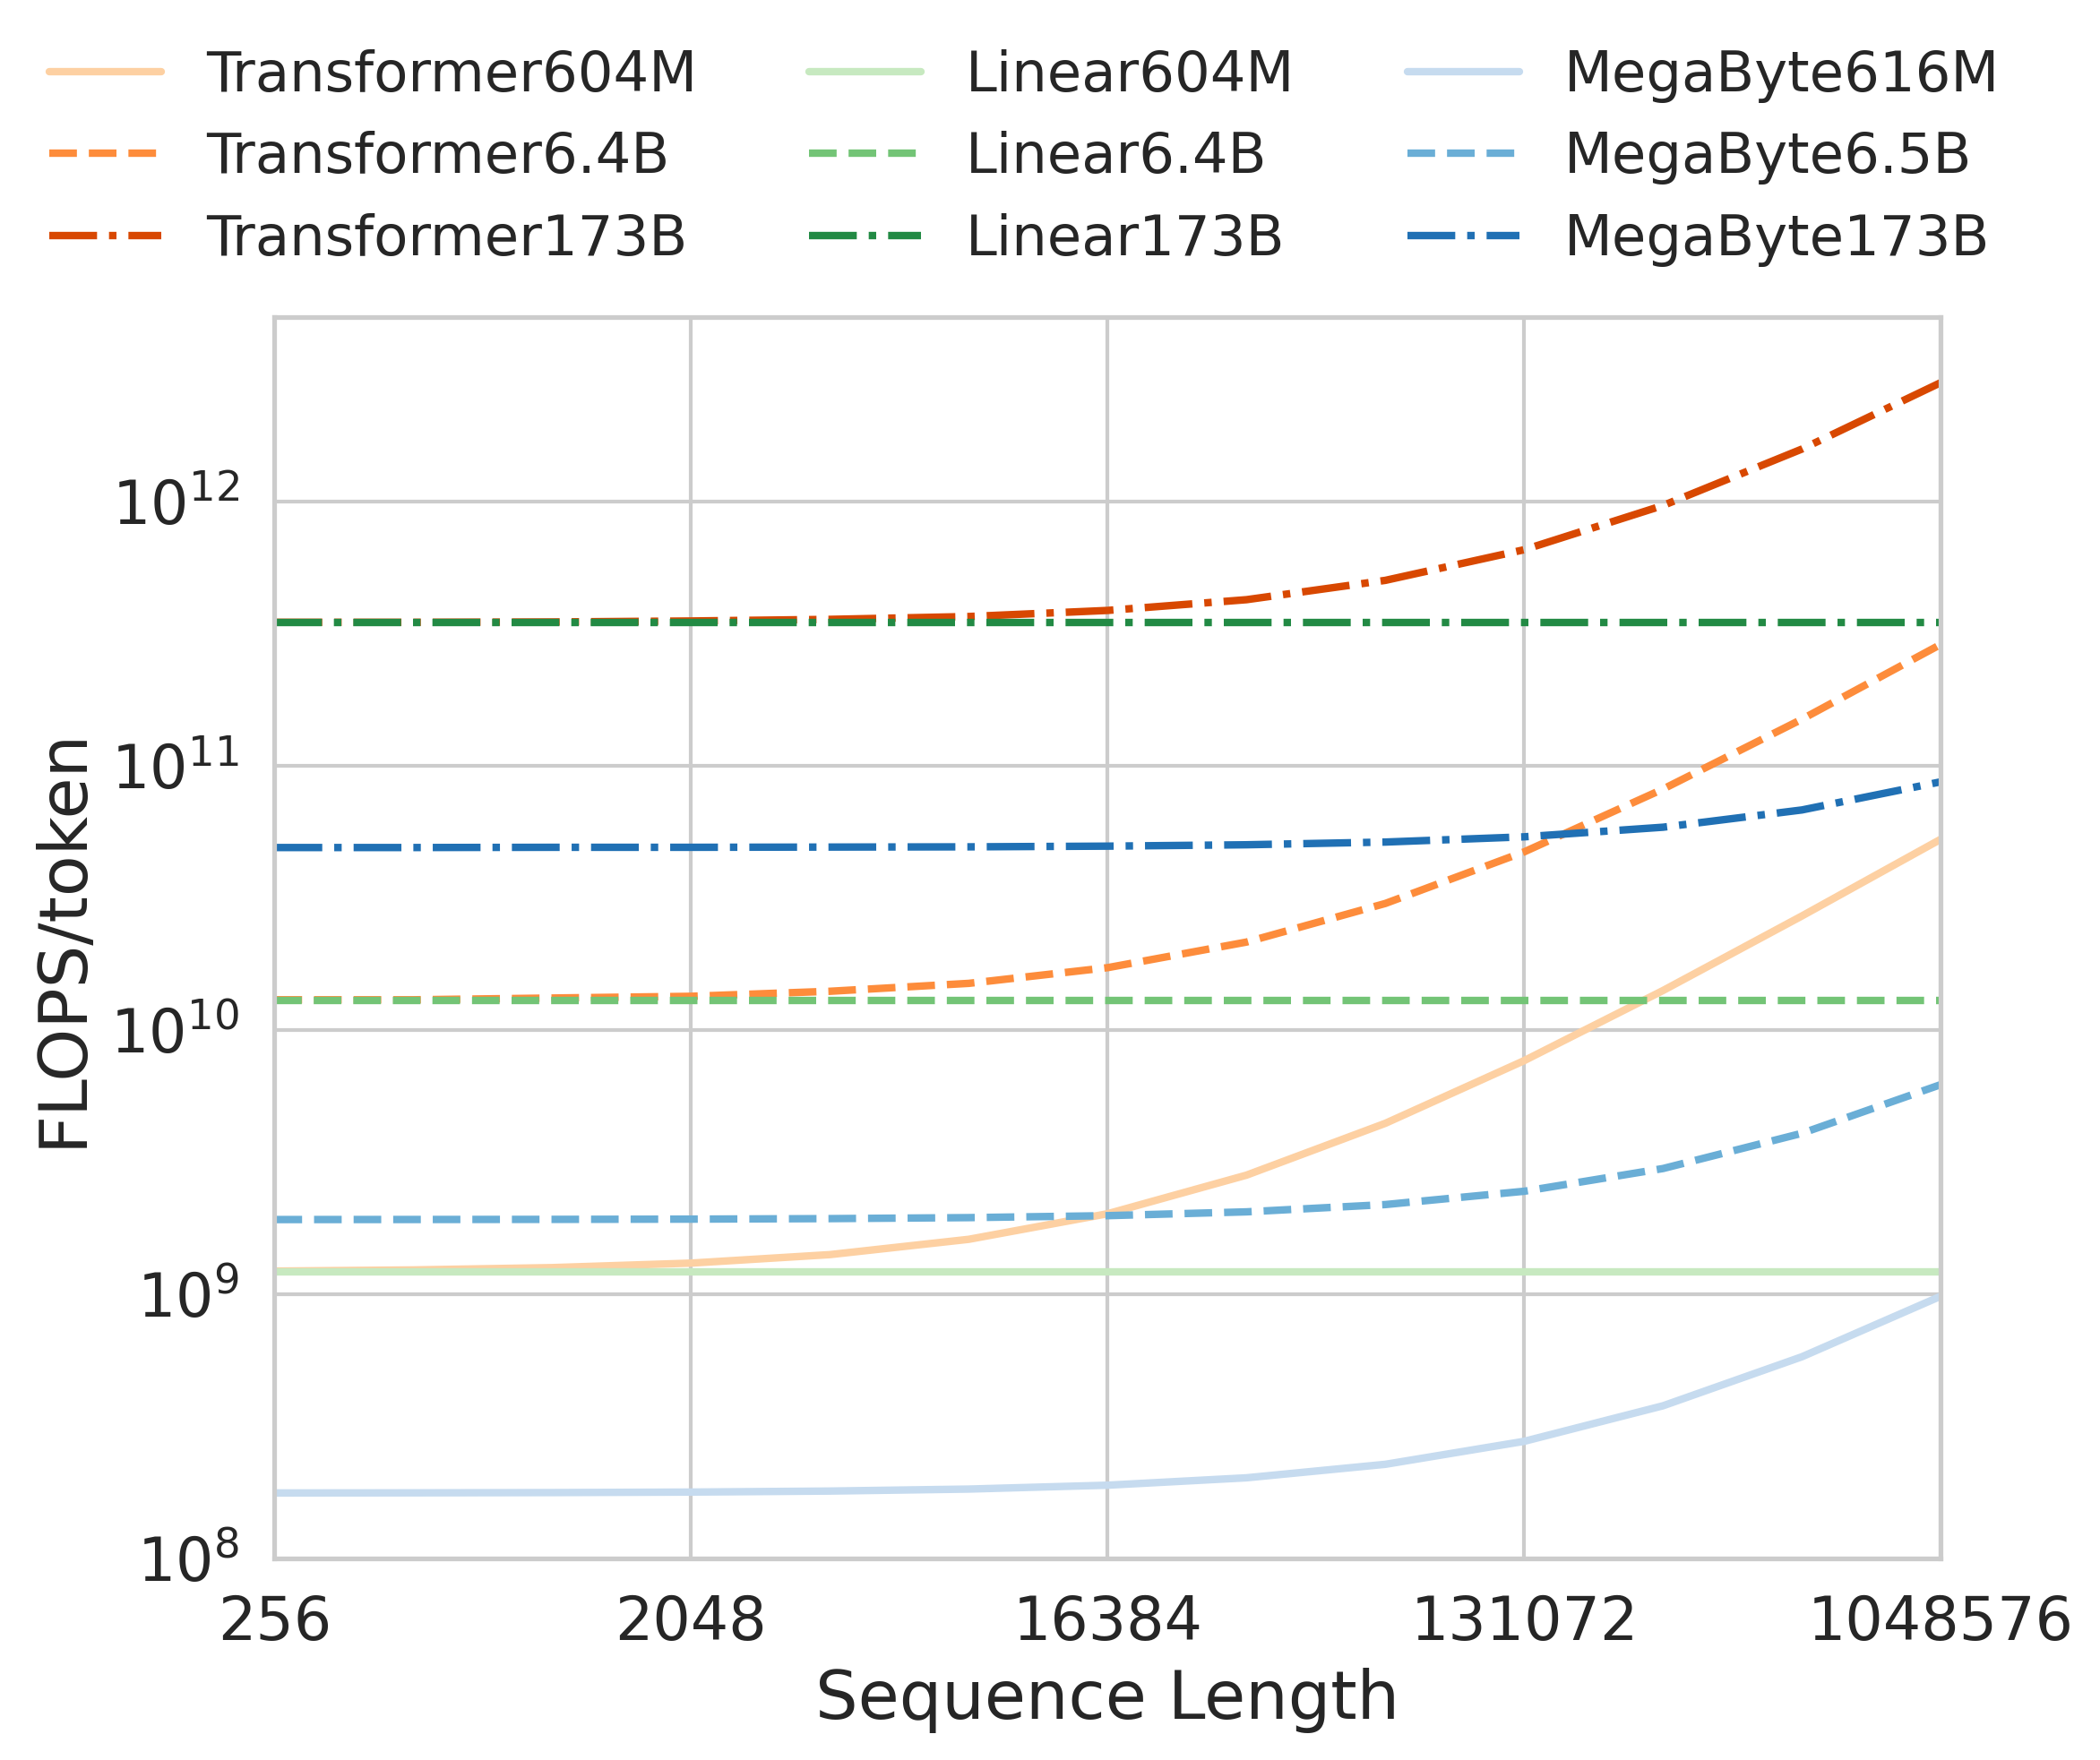
\includegraphics[width=\linewidth]{figs/flops.png}
\caption{\label{figure:flops}Computational cost (FLOPS/token) for different model architectures at different scales. \megabyte architectures (here with $P=8$) use less FLOPS than equivalently sized Transformers and Linear Transformers~\citep{lineartransformer} across a wide range of model sizes and sequence lengths, allowing larger models to be used for the same computational cost.}
\end{figure}

\paragraph{Combined Analysis} To understand efficiency at different sequence lengths and model sizes, we calculate the total FLOPS used by transformers, Linear Transformers and \megabyte. For each operation, we use FLOP estimates from \citep{kaplan2020scaling}, except for attention in Linear Transformers, which we estimate as $9D$ FLOPS/token\footnote{This may underestimate the time taken by Linear Transformer decoders, which use a recurrence mechanism that is harder to parallelize on current hardware.}, where $D$ is the model embedding dimension. Figure \ref{figure:flops} shows that for models of size 660M to 173B and sequence lengths of up to 1M tokens, \megabyte with $P=8$ uses less FLOPS than either transformers or Linear Transformers. Baseline model architectures are based on GPT3, and Megabyte global/local model sizes are 452M/151M, 5.8B/604M, 170B/3.2B respectively.


%By dividing long sequences into patches, our slow model uses a factor of $p$ less compute than an equivalent vanilla transformer, or even linear transformer. This property allows us to train larger models for the same cost.

%An important component of evaluating the quality of a language model architecture is understanding its training efficiency as a function of scale, both in model size and sequence length. In particular, we are interested in the scaling efficiency of \megabyte in comparison to a standard decoder-only Transformer. Reasoning about the training efficiency of \megabyte is not that difficult given that it is essentially a combination of two Transformers. From an asymptotic perspective and given an input sequence of length $n$ from which to decode a next token, a Transformer has time complexity of $O(n^2)$; whereas \megabyte with patch size $p$ has time complexity $O(\frac{n}{p}^2 + np^2)$. In practice, parallelism techniques imply that varying slow and fast model sizes can introduce different compute bottlenecks into the overall training and inference pipelines. Generally speaking, ... we 


\subsection{Generation Efficiency}
Generating long sequences with transformers is slow, because the input to each timestep is the output from the previous timestep, meaning each layer must be computed for each token serially. As running a layer on a single token typically does not saturate the amount of parallelism available within a GPU, for analysis, we model each layer as a constant cost independently of size. Consider a \megabyte model with $\Lglobal$ layers in the Global model and $\Llocal$ layers in the Local model and patch size $P$, compared with a Transformer architecture with $\Llocal+\Lglobal$ layers. Generating each patch with \megabyte requires a sequence of $O(\Lglobal+P\cdot \Llocal)$ serial operations, whereas the Transformer requires $O(P\cdot \Lglobal+P\cdot \Llocal)$ serial operations. When $\Lglobal\gg \Llocal$ (i.e. the Global model has many more layers than the Local model), \megabyte can reduce inference costs by a factor close to $P$.



\section{Experimental setup}
\label{sec:exp}

\subsection{Controlling for Compute and Data}
    \label{sec:controlled_exp}
Models show consistent improvements when increasing both data and compute \cite{kaplan2020scaling,Chinchilla}, meaning that one model can outperform another because of an increased training budget instead of an improved architecture. However, in practice, both compute and data are typically limited. We conduct experiments using a fixed compute and data budget across all models to focus comparisons solely on the model architecture rather than training resources. To achieve this, we adjust model hyperparameters (mainly, number of layers) within each architecture so that the forward pass time taken per byte is matched, and then train all models for the same number of bytes.


\subsection{Comparison Systems}
We compare \megabyte with both a standard decoder-only Transformer and PerceiverAR \citep{perceiverar}. PerceiverAR extends the original transformer with a single cross-attention layer over a much longer context sequence, and is the best performing general purpose autoregressive model we are aware of 
 and achieves state-of-the-art results across several modalities. We implemented both models in the same codebase, and all models share a similar data loader, preprocessing step, and trainer to avoid any artifacts in our compute-controlled experiments.



\subsection{Training Procedure}
    \label{sec:training_proc}
    All models were trained using the Metaseq\footnote{https://github.com/facebookresearch/metaseq} code base~\cite{OPT}. The training used the PyTorch framework \cite{pytorch}, with fairscale to improve memory efficiency through fully sharded model and optimizer states \cite{fairscale}. Mixed precision training was used to improve training efficiency at scale \cite{mixedprecision}. More training details and various model parameters can be found in Section \ref{subsec:append_training} in the Appendix. 

To validate our implementation of PerceiverAR, we reproduced their experiments on downsized ImageNet at 64 pixels. By carefully matching hyperparameters, we achieved a bits per byte (bpb) score of 3.53, compared to the reported 3.54 in the original paper.

\subsection{Inference Methods}
Several techniques have been proposed for trading off speed for performance during inference with language models, including sliding windows \cite{shortformer} and our strided inference (Section \ref{strided}). We only use these methods when comparing with prior published work (Tables \ref{tab:text_sota} and \ref{tab:img_sota}).




\section{Language Modeling}
We evaluated the performance of \megabyte on language modeling on a set of 5 diverse datasets emphasizing long-range dependencies: Project Gutenberg (PG-19), Books, Stories, arXiv, and Code. 
%We are also interested in the effectiveness of \megabyte on text modalities, in which long-range connections play an important role. Examples include natural language documents such as books, source code, and technical publications like this one. To this end, we tested our model on 5 datasets: Project Gutenberg (PG-19), Books, Stories, arXiv, and Github. 
\begin{table}[t]
    \centering\small
    \begin{tabular}{lrr}
    \toprule
    Dataset & Total Bytes & Mean document size (bytes)  \\
    \midrule
    PG-19 & 10.1GB & 411,404 \\
    Stories & 21.3GB & 35,265 \\
    Books & 79.7GB & 509,526 \\
    arXiv & 91.5GB & 58,518 \\
    Code & 353.7GB & 7,461 \\
    \bottomrule
    \end{tabular}
    \caption{Text dataset sizes and mean document lengths.}
    \label{tab:document_lengths}
\end{table}





\textbf{Datasets} We experiment on a range of long form text datasets. The PG-19 dataset \cite{pg19} consists of English-language books written before 1919 and is extracted from the \href{https://www.gutenberg.org/}{Project Gutenberg online library}. The Stories dataset \cite{stories} is a subset of CommonCrawl data meant to emulate Winograd schemas. Books \cite{pile} is another collection of English-language books. The arXiv dataset is a collection of technical publications written in \LaTeX ~from the \href{arxiv.org}{arXiv online archive}. Finally, the Code dataset is a large publicly available dataset of open source code, under Apache, BSD or MIT licenses. More details on dataset sizes and document lengths are shared in Table \ref{tab:document_lengths}. 

\begin{table}[t]
\centering\small
\begin{tabular}{l|ccccc}
\toprule
& PG-19 & Stories & Books & arXiv & Code \\
\midrule
% Books run is done and in spreadsheet. Add from there.
Transformer & 1.057 & 1.064 & 1.097 & 0.816 & 0.575 \\
PerceiverAR & 1.104 & 1.070 & 1.104 & 0.791 & 0.546 \\
\megabyte & \textbf{1.000} & \textbf{0.978} & \textbf{1.007} & \textbf{0.678} & \textbf{0.411} \\
\bottomrule
\end{tabular}
\caption{Performance (bits-per-byte) of compute and data controlled \megabyte, PerceiverAR, and Transformer models on various text modalities. }
\label{tab:text_exps}
\end{table}


\textbf{Controlled Experiments} Table \ref{tab:text_exps}, lists bpb on each dataset. Each model is trained for 80 billion bytes, and models are scaled to use the same compute budget. We carefully tune hyperparameters for all architectures to best utilize the available compute budget. \megabyte consistently outperforms both baseline transformers and PerceiverAR across all datasets. We use the same set of parameters on all datasest. In all experiments presented in Table~\ref{tab:text_exps}, transformer has size of 320M with context length of 1024, PerceiverAR has size of 248M with context size of 8192 and latent size of 1024, and \megabyte global/local model sizes are 758M/262M with context length of 8192 and patch size of 8. %In this compute and data-controlled setting, we observe limited gains from PerceiverAR over the baseline transformer for some datasets, but much larger improvements from \megabyte. 




\begin{table*}[t]
\centering
\small
\begin{tabular}{lccccc}
\toprule
{} & Tokenizer & Vocab Size & Context Length & Validation & Test \\
\midrule
TransformerXL          \cite{compressive}       & SentencePiece & 32k & 512+1024 (subwords) & 45.5 & 36.3 \\
CompressiveTransformer \cite{compressive}       & SentencePiece & 32k & 512+512+2x512 (subwords) & 43.4 & 33.6 \\
PerceiverAR \cite{perceiverar}   & SentencePiece & 32k & 2048 (subwords) & 45.9 & 28.9 \\
BlockRecurrent \cite{blockrecurrent}            & SentencePiece & 32k & 1024+recurrence (subwords) & -   & \bf{26.5} \\
\midrule 
%BlockRecurrent byte-level \cite{blockrecurrent} & Bytes         & 256 &  &  46.6\\
Transformer byte-level (ours)                   & Bytes         & 256 & 2048 (bytes) & 81.6 & 69.4  \\
PerceiverAR byte-level (ours)                   & Bytes         & 256 & 8192 (bytes) & 119.1 & 88.8 \\
\megabyte                                       & Bytes         & 256 & 8192 (bytes)  & \bf{42.8} & 36.4 \\
% \hspace{5pt} \textit{w/o slow model}  & x.xx & 3.181 & x.xx \\
% \hspace{5pt} \textit{w/o pre context}  & x.xx & \wip{3.248} & x.xx \\
\bottomrule
\end{tabular}
\caption{\label{tab:text_sota}Larger scale experiments on PG19, converting bits-per-byte to word-level perplexities for comparison with prior work. Results below the line are compute-matched.  \megabyte outperforms other byte models by a wide margin, and gives results competitive with state-of-the-art models trained on subwords.}
% \caption{Larger scale experiments on PG19, with only results below the line controlled for compute or tuning, and converting bits-per-byte to word-level perplexities for comparison with prior work. \megabyte outperforms other byte models by a wide margin\footnote{The only prior byte-level experiments we are aware of are at a smaller scale in \citet{blockrecurrent}, who report results equivalent to test perplexities of 46.5 with a version of the BlockRecurrent transformer, and 49.5 with Memorizing Transformers \cite{memorizing}, compared to 36.4 with our model. }, and gives results competitive with state-of-the-art models trained on subwords.}
\label{tab:pg19_summary}
\end{table*}
\label{sec:results}


\textbf{Scaling Experiment} We scale up our training data on PG-19 (Table~\ref{tab:pg19_summary}), and compare \megabyte with byte baselines, as well as converting all results to word-level perplexities to benchmark with state-of-art token based models. 

We train a byte-level Transformer, PerceiverAR and \megabyte models for 400B bytes and the same compute budget using same model parameters as in the controlled experiments. We find that \megabyte outperforms other byte-level models by a wide margin at this scale.\footnote{The only prior byte-level experiments we are aware of are at a smaller scale in \citet{blockrecurrent}, who report results equivalent to test perplexities of 46.5 with a version of the BlockRecurrent transformer, and 49.5 with Memorizing Transformers \cite{memorizing}, compared to 36.4 with our model. } %with a 262M parameter Local model and 758M parameter Global model for 400 billion bytes. 

We also compare with the best previously reported numbers for sub-word models. These results may be confounded by differing amounts of compute and tuning used, but show that \megabyte %outperforms other byte models by a wide margin, and 
gives results competitive with state-of-the-art models trained on subwords. These results suggest that \megabyte may allow future large language models to be tokenization-free.



\section{Image Modeling}
\label{sec:image}

\subsection{Sequence Modeling on ImageNet}



We test \megabyte on variants of the autoregressive image generation task on ImageNet \citep{Oord2016PixelNetworks}, to measure its ability to efficiently use long context. We test on three different resolutions of images, ranging from 64\texttimes64 to 640\texttimes640 pixels -- the latter requiring the effective modeling of sequences with over 1.2M tokens. This generation task becomes increasingly challenging as the image's resolution grows: doing well on this task requires the modeling of local patterns (textures, lines, etc.) and long-range context that provides information about the high level structure of the image. Inspired by recent works in Vision Transformers~\citep{vit}, we model image data patch by patch (more details can be found in Appendix~\ref{sec:scan_type}). 


%Unless otherwise noted, \megabyte models scan bytes by first dividing an $\sqrt{T}\times \sqrt{T}$ image into $K$ patches of size $\sqrt{P} \times \sqrt{P}$ such that $T=KP$, then applying raster scan in each patch sequentially as illustrated in Figure \ref{fig:scan}. This scanning method does not impact the autoregressive nature of the task as we scan all pixels in a fixed order every time. 
% \todo{Run ablation for raster scan ordering}



%\subsection{Controlled Experiments}

\subsection{Comparison with State of the Art}

%Perceiver AR \citep{HawthorneGeneral-purposeAR} is a general purpose autoregressive model that uses a single cross-attention layer over a long range context in order to represent it in a fixed number of latent representations, yielding state-of-the-art performance on the ImageNet 64\texttimes 64 autoregressive image generation task \footnote{\url{https://www.tensorflow.org/datasets/catalog/downsampled_imagenet} }.

We train a large \megabyte model on ImageNet 64x64 with Global and Local models sized 2.7B and 350M parameters, respectively, for 1.4T tokens. We estimate that training this model consumed less than half the GPU hours we would have needed to reproduce the best PerceiverAR model described by \citep{perceiverar}. %We use a \textit{strided} evaluation technique that combines outputs from two forward passes per image to produce optimal performance - in a manner similar to the sliding window evaluation used by PerceiverAR. More details on this method are provided in Section \ref{strided_inference}. 
As shown in Table \ref{tab:img_sota}, \megabyte matches the state-of-the-art performance of PerceiverAR whilst using only half the compute.

 % \mike{is this really the 'strided evaluation'?}

\begin{table}[h]
\centering
\begin{tabular}{lr}
\toprule
{ImageNet64} & \bpb\\
\midrule
Routing Transformer \citep{routing} & 3.43 \\
Combiner \citep{combiner} & 3.42 \\
Perceiver AR \citep{perceiverar} & \textbf{3.40}  \\
\megabyte &  \textbf{3.40} \\
\bottomrule
\end{tabular}
\caption{Bits per byte (\bpb) on ImageNet 64\texttimes 64.  \megabyte matches the current state-of-the-art while only using half the amount of GPU hours to train.}
\label{tab:img_sota}
\end{table}


\subsection{Scaling to higher resolutions}

%Since recent literature (e.g. ~\citep{Chinchilla}) suggests that large pre-trained models are not bottlenecked by their number of parameters but rather by compute and data, we adjust the hyperparameters of each model (e.g. context size, number of parameters, number of latents) such that
% To push the limits of long sequence modeling, we also explore higher resolution images.
We compare three transformer variants (vanilla, PerceiverAR, \megabyte) to test scalability to long sequences on increasingly large image resolutions. We use our own implementations of these in the same framework and budget the same amount of GPU hours and data to train each of these model variants. 

%Transformer baselines use 2048 sequence length and PerceiverAR baselines use 1024, \todo{XX}, \todo{XX} latents with overall context size of 12K, \todo{XX}K, \todo{XX}K for the three image resolutions respectively. \todo{add details?}. 
\megabyte is able to handle all sequence lengths with a single forward pass of up to 1.2M tokens. We found neither the standard Transformer nor PerceiverAR could model such long sequences at a reasonable model size, so instead we split images into segments of size 1024 and 12000 respectively.
For Megabyte, we set patch size as 12 for Image64 and patch size as 192 for Image256 and Image640 datasets. Model sizes are adjusted to match overall training speeds across models and we do not use any form of sliding window evaluation in this experiment. As seen in Table \ref{tab:resolution_scale}, \megabyte outperforms baselines across all resolutions in this compute-controlled setting.
The precise settings used for each of the baseline models  such as context length and number of latents are summarized in Table \ref{table:opt_model_desc}.

Results show that \megabyte outperforms the other systems at all resolutions, demonstrating an effective model of sequences of over 1M bytes.

%Using the same method for matching compute and data we also run ablations to determine the role of various components. In Table \ref{tab:text_ablations_256} we show that all components contribute meaningfully to the performance of \megabyte.
%We experiment with: 1) replacing the fast model with a simple dense layer to produce the output tokens based on the slow model output and 2) using only the slow model output as input to the fast model without additional context tokens. \todo{Formalize this with notation from Section 2 after it is finalized}

\begin{table}[t]
\centering
\small
\begin{tabular}{lrrrr}
\toprule
{} & Context & Image64 & Image256 & Image640 \\
\midrule
% Pixels & & 64x64 & 256x246 & 640x640 \\
Total len & & 12288 & 196608 & 1228800 \\
\midrule
Transformer & 1024 & 3.62 & 3.801 & 2.847 \\
Perceiver AR & 12000 & 3.55 & 3.373 & 2.345 \\
\midrule
\megabyte & Full & \textbf{3.52} & \textbf{3.158} & \textbf{2.282} \\
\bottomrule
\end{tabular}
\caption{Bits per byte (\bpb) on ImageNet with different resolutions. All models use the same compute and data. MEGABYTE scales well to sequences of over 1M tokens.
\label{tab:resolution_scale}}
\end{table}


\section{Audio Modeling}
\label{sec:speech}

% We evaluate our speech model by testing its ability to generate speech byte by byte, and conduct experiments on several different datasets. Specifically, we test our model on the following datasets:

Audio has aspects of both the sequential structure of text and the continuous nature of images, so is an interesting application for \megabyte.
%We evaluate our speech model by testing its ability to generate speech byte by byte, and conduct experiment on LibriLight-Large~\citep{librilight} dataset.
% \paragraph{LibriLight-Large~\citep{librilight}}
%The LibriLight-Large dataset contains an extensive collection of 60,000 hours of unlabelled speech from audiobooks in English. The dataset includes 3,509,146 audio clips, each with an average duration of 52 seconds. We randomly split out the training and validation set.

% \paragraph{Spotify-60K~\citep{spotify}}
% The Spotify Podcast dataset includes 100,000 episodes from various podcast shows on Spotify, with approximately 60,000 hours of English audio data. Over 90\% of the podcasts feature two- or three-person conversations. All audio clips are clipped to an average length of 35 seconds. 

Raw audio is typically stored as a sequence of 16-bit integer values (one per timestep); a softmax layer would need to output 65,536 probabilities per timestep to model all possible values. To address this issue, various techniques have been developed to reduce the memory and computational requirements of the softmax layer. For instance, \citet{wavenet} apply $\mu$-law companding transformation and quantizes the input into 256 possible values. Alternatively, \citet{parawavenet} model the samples using the discretized mixture of logistics distribution introduced by \citet{pixcelcnn++}. Finally, \citet{wavernn} use a dual softmax technique to produce 8 coarse and 8 fine bits. In our approach, we simplify the audio modeling process by directly reading the bytes (256 possible values) from the audio file and conducting an autoregressive language model on top of that. This greatly streamlines the modeling process, making it easier and more efficient.

Our audio modeling approach focuses on 16 kHz, 16-bit audio, which equates to 32k bytes per one-second clip. We use an extensive audio dataset consisting of 2 terabytes (roughly 18,000 hours) of audio. We use a sequence length of 524,288, a patch size of 32, and a batch size of 32 to facilitate model training. By utilizing these settings, we can effectively train our model on large volumes of audio data, helping to improve its accuracy and efficacy.

Our model obtains bpb of 3.477, much lower than the results with perceiverAR (3.543) and vanilla transformer model (3.567). More ablation results are presented in Table \ref{tab:ablations}. 



\section{Analysis}
\subsection{Generation speed}

We also compare the text generation speed between \megabyte and a transformer. %We ran controlled experiments on PG19 and train both models with the same GPU hours. 
We compare a 350M parameter baseline transfomer and a \megabyte model with a 1.3B parameter Global model and a 218M parameter local model, trained on PG19 with equal compute.
As shown in Table~\ref{tab:generation}, the \megabyte model achieves much lower perplexity as expected.
However, \megabyte also generates a sequence of 8192 tokens 40\% \emph{faster} than transformer, despite having over 4 times the parameters.
This speed up is due to the bulk of the parameters being in the Global model, which only needs to be computed once for every 8 tokens, whereas all the parameters in the baseline model are used on every token.

\begin{table}[t]
    \centering\small
    \begin{tabular}{ccccc}
    \toprule
& \makecell{Global\\Size} & \makecell{(Local)\\Size} & \makecell{\bpb\\} & \makecell{Generation\\Time (s)} \\
    \midrule
Transformer    &- & 350M & 1.064 & 132 \\ % ~(D=1024,L=24)
\megabyte & 1.3B & 218M & 0.991 & 93 \\ % ~(D=1024,L=15)
    % \midrule
    % 192 & 125M & 125M (D=768, L=12) & 3.215\\
    % 192 & 350M & 350M (D=1024, L=24) & 3.209 \\
    % 192 & 1.3B & 125M (D=768, L=11) & 3.205 \\
    \bottomrule
    \end{tabular}
    \caption{Comparison of bits per byte (bpb) and generation speed of 8192 bytes of transformer model (with context length 1024) and \megabyte with context length 8192 and patch size 8.}
    \label{tab:generation}
\end{table}



\subsection{Model Components}
In Table \ref{tab:ablations}, we  analyze the significance of different components in the \megabyte architecture by studying arXiv, Librilight-L and ImageNet256 datasets. 
% In the second to last row \todo{rewrite}, we remove cross-patch attention from the Local model with a vanilla Transformer model, illustrating the importance of inter-patch attention for short-range connection modeling. In the final row, we explore a convolutional neural network as the neural patch encoder. Unlike the simpler concatenation approach, it can contextualize patch embeddings with both information on intra-patch byte connections and information on connections with nearby patches.
Removing Local (\textit{w/o local model}) or global (\textit{w/o global model}) model, we observe a substantial increase in bpb on all datasets, showing that both parts are crucial. 
The performance of the model without the cross-patch local model (\textit{w/o cross-patch local model}) is competitive, indicating that the architecture is robust to this modification.
We observe slight improvement on the Librilight-L and ImageNet256 datasets by augmenting the \megabyte model with a CNN encoder (\textit{w/ CNN encoder}). This suggests that the \megabyte architecture can benefit from integrating alternative encoding mechanisms.


\begin{table}[h!t]
\centering\small
\begin{tabular}{lrrr}
\toprule
{}  & Arxiv & Audio & ImageNet256  \\
\midrule
% Transformer  & 0.816 & 3.567 & 3.801\\
% Perceiver AR & 0.791 & 3.543 & 3.373\\
% \midrule
\megabyte    & 0.6871 & \textbf{3.477} & \textbf{3.158}\\
%\hspace{5pt} \textit{w/ strided inference}  & & & \\
\hspace{2pt} \textit{w/o local model}  & 1.263 & 5.955 & 4.768\\
\hspace{2pt} \textit{w/o global model}  & 1.373 &  3.659  & 3.181\\
\hspace{2pt} \textit{w/o cross-patch attention}  & \textbf{0.6781} & 3.481 &3.259 \\
\hspace{2pt} \textit{w/ CNN encoder}  & 0.6871 & \textbf{3.475} & \textbf{3.155}\\
\bottomrule
\end{tabular}
\caption{Ablation of \megabyte model components, showing that both Local and Global models are critical to strong performance, but the architecture is robust to other modifications. We report bits-per-byte on text, audio, and image prediction tasks. All models within a column are trained using the same compute and data. The hyperparameters are listed in Table \ref{table:opt_model_desc}. }
\label{tab:ablations}
\end{table}




\subsection{Effective Use of Context}
Long-context models often struggle to benefit from the full context \citep{sun2021long}. Figure \ref{fig:prob_within_context} shows that later tokens within each context window consistently have a higher likelihood, indicating that \megabyte can effectively use at least 8k bytes of context on the PG19 dataset. 
% This property also makes it possible for \megabyte to benefit from sliding window evaluation - as demonstrated by the first two rows of Table \ref{tab:inference_options}. \mike{I don't follow the last sentence, other models benefit from sliding windows too?}

 \begin{figure}[t]
    \centering
    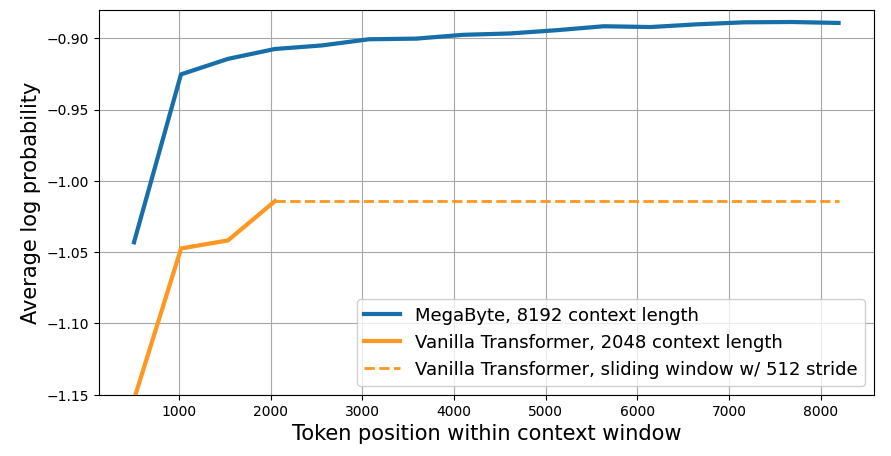
\includegraphics[width=\linewidth]{figs/probs_within_context_baseline_sliding_window.png}
    \caption{Average log probability assigned to the token at different positions within the context length by \megabyte model with 8192 context size and by a vanilla transformer model trained using the same compute (PG19 test set). 
    \megabyte likelihoods rise throughout its context window, demonstrating that it can use tokens from 8k bytes previously to improve its predictions.
    %\megabyte is able to benefit from at least 8192 tokens of context with a single inference, while the sliding window evaluation for a vanilla transformer can only have limited benefits even at an increased inference cost.
    }
    \label{fig:prob_within_context}
\end{figure}

%\mike{Can we also graph some compareable baseline models?}

\subsection{Strided Inference}
\label{strided_inference}
 We find that within a single patch, on average, the \megabyte performs worse on later tokens within a patch (see Figure \ref{fig:strided_inference}). 
 % This result is likely because the Global model does not have access to earlier tokens within each patch. 
 Section \ref{strided} proposes \emph{strided inference} as a solution, where two forward passes are performed offset by $\frac{P}{2}$ tokens, and results from the first half of each patch are combined.
 Table \ref{tab:inference_options} shows performance improvements from strided inference, which are additive with the standard sliding window.

\begin{figure}[t]
    \centering
    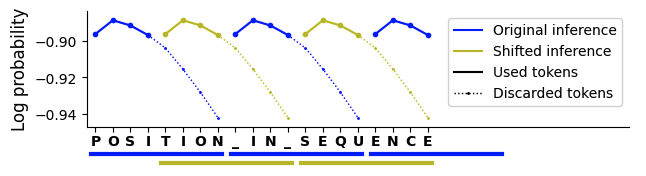
\includegraphics[width=\linewidth]{figs/strided7.png}
    \caption{An illustration of strided inference with patch size 8. Lines below the text represent the patches used in the two rounds of inference, the plot above it represents the average probability assigned to the token at a given position within a patch. By considering only the first half of each patch from the two rounds of inference and combining them (bold lines on top), we achieve a better overall \bpb.}
    \label{fig:strided_inference}
\end{figure}

%\mike{Replace x-axis with something like: Position in sequence}

%Analogously to sliding window evaluation - which increases the average context available for traditional LMs by doing multiple rounds of inference - we use \emph{strided inference} to further improve the performance of \megabyte (see Section \ref{section:strided}). In a second round of inference we offset bytes by $\frac{P}{2}$ such that tokens that were originally in the second half of a patch now belong to the first half. We then combine token probabilities from these two inferences by taking blocks of $\frac{P}{2}$ tokens alternating between the two outputs - resulting in improved bpb. We illustrate this method in Figure \ref{fig:strided_inference} and show benefits of it in Table \ref{tab:inference_options}. Note that one can also use this technique together with sliding window evaluation, resulting in further gains in performance.





\begin{table}[t]
    \centering\small
    \begin{tabular}{lcc}
    \toprule
    Method & Inference Cost & bpb \\
    \midrule
    Basic Inference & 1X & 0.9079 \\
    \hspace{2pt} \textit{w/ Sliding Window} & 2X & 0.8918 \\
    \hspace{2pt} \textit{w/ Strided Inference} & 2X & 0.8926 \\
    \hspace{2pt} \textit{w/ Sliding \& Strided} & 4X & \textbf{0.8751} \\
    \bottomrule
    \end{tabular}
    \caption{Performance of various inference techniques on the PG19 test set using our best \fastslow model.}
    \label{tab:inference_options}
\end{table}

\subsection{Hyperparameters}

\megabyte introduces several additional hyperparameters. We tuned these parameters independently for different modalities and reported performance based on the best setting we found. All experiments in the same group use the same compute. 
% In this section, we use one of the modalities - Image256 - to analyze the role of two important hyperparameters: Local / Global model size ratio and Patch Size. Since these parameters impact the compute cost of our models, we slightly adjust the number of transformer layers in the Local model to ensure all versions consume the same amount of compute. We summarize our results in Table \ref{tab:hyperparams_ablation}.

%\mike{Are the layer/param numbers right?}
% Daniel: yes. Slow model is very cheap for image since our patch size is larger.

\textbf{Patch Size.} We experimented with various patch sizes on Image256 dataset and found that there is a wide range of values where \megabyte performs similarly. We found similar robustness against the choice of this hyperparameter across all modalities, although the optimal patch size itself can be different across modalities.

\begin{table}[h]
    \centering\small
    \begin{tabular}{cccc}
    \toprule
    Patch Size & Global Size & Local Size & \bpb \\
    \midrule
    48 & 125M & 114M~(D=768, L=11)  & 3.178 \\
    192 & 125M & 125M~(D=768, L=12)  & 3.158 \\
    768 & 125M & 83M~(D=768, L=8) & 3.186 \\
    % \midrule
    % 192 & 350M & 350M (D=1024, L=24) & 3.209 \\
    % 192 & 125M & 350M (D=1024, L=24) & 3.215\\
    % 192 & 1.3B & 350M (D=1024, L=23) & 3.205 \\
    % \midrule
    % 192 & 125M & 125M (D=768, L=12) & 3.215\\
    % 192 & 1.3B & 125M (D=768, L=11) & 3.205 \\
    \bottomrule
    \end{tabular}
    \caption{Effects of patch size on performance on the Image256 dataset. All versions use the same amount of GPU hours and data.}
    \label{tab:hyperparams_ablation}
\end{table}


\textbf{Local to Global model Size Ratio.} We experimented with different Local/Global model size ratios on PG19 dataset. By grouping bytes into patches, \megabyte effectively uses $P$ times less tokens for the Global model as on the Local model---enabling us to increase the size of the Global model without reduced cost. We find that a given compute budget is spent optimally when the Global model has more parameters than the Local model. This trend was consistent across all modalities and various patch sizes.

\begin{table}[t]
    \centering\footnotesize	
    \begin{tabular}{ccc}
    \toprule
    Global Size & Local Size & \bpb \\
    \midrule
   350M~(D=1024,L=24)  & 290M~(D=1024,L=20) & 1.014  \\
    760M~(D=1536,L=24) & 262M~(D=1024,L=18) & 1.002  \\
    1.3B~(D=2048,L=24)  & 218M~(D=1024,L=15) & 0.991  \\
    % \midrule
    % 192 & 125M & 125M (D=768, L=12) & 3.215\\
    % 192 & 350M & 350M (D=1024, L=24) & 3.209 \\
    % 192 & 1.3B & 125M (D=768, L=11) & 3.205 \\
    \bottomrule
    \end{tabular}
    \caption{Effects of Local / Global model size on performance on the PG19 dataset. Increasing the capacity of global model improves performance. Models are compute and data matched.}
    \label{tab:size_inference}
\end{table}




\section{Related Work}
\label{sec:related}
Prior research has explored the possibility of improving the efficiency of Transformers on long sequences, primarily motivated by mitigating the quadratic cost of self-attention.

\textbf{Efficient Encoder Models} Several related techniques to ours have been developed for transformer encoder architectures but cannot be straightforwardly applied to decoders. In particular, patchifying operations have previously been used in image \emph{encoder} models such as ViT \citep{vit}, and down- and up-sampling operations have been used for text encoders \citep{canine}, but such methods cannot be naively applied to decoder-only models without leaking information to future bytes in the same patch. \megabyte generalizes these approaches to an efficient decoder model by using a intra-patch transformer to predict each sequence element's likelihood, and offseting the inputs to the two models to avoid leaking information. \citet{perceiver} which uses self-attention on a shorter latent sequence, and \citet{temporalbottleneck} which uses recurrent model to process chunks with $k$ input steps also resemble patchification, but this technique cannot easily be applied to decoder architectures without leaking information to future timesteps.

\textbf{Efficient Decoder models} Improving the efficiency of decoder models is more challenging because of the need to make one prediction per timestep, and not leak information to future timesteps. The most popular approaches can be categorized as (1) chunking sequences into smaller blocks, and propagating information from previous blocks with either recurrence \citep{xfmxl,blockrecurrent} or cross-attention \citep{perceiverar}, (2) linear alternatives to attention, which typically involve forms of token-level recurrence \citep{lineartransformer, linear} or state space models \citep{s4,s5,mega}, or (3) sparse approximations of attention \citep{reformer,longformer,sparsetransformer,memorizing}. However, the performance of dense attention means it is typically still chosen for large scale decoders \citep{llama,palm}. \megabyte takes the alternative approach of decomposing the complete sequence into two shorter sequences, giving sub-quadratic attention. We also note that feedforward networks are the dominant cost in large decoders, not self-attention. Our approach to compressing sequences allows much larger models than would be possible when using large feedforward networks at every timestep.

\textbf{Tokenization} The most common approach to shortening sequence lengths in Transformer decoders is to pre-process the input with a form of tokenization, in which multiple bytes are mapped to a single discrete token from a fixed vocabulary. For text, this can be done losslessly using methods such as BPE \citep{bpe} and SentencePiece \citep{sentencepiece}, but these approaches can require language-specific heuristics \citep{gpt2}, limit out-of-domain performance \citep{sharami2023systematic}, and can affect prompting and truncated sampling in unpredictable ways.\footnote{For example, whether or not a prompt should end in whitespace depends on details of the underlying subwod algorithm used.} \citet{subword} downsamples characters using subword information and has shown promising results in machine translation tasks. The amount of high-frequency information in images and audio means that tokenization cannot be performed losslessly, and instead clustering \citep{hubert} or discrete auto-encoders \citep{dalle} are used to compress the inputs, which lose information and likely limit generative model performance. Our patches are analogous to traditional lossless tokens, and the Local model performs the role of mapping a hidden state to a distribution over possible patches.

\section{Conclusion}
We introduced \megabyte, a scaleable architecture for modeling long sequences.
\megabyte outperforms existing byte-level models across a range of tasks and modalities, allowing large models of sequences of over 1 million tokens.
It also gives competitive language modeling results with subword models, which may allow byte-level models to replace tokenization.
However, the scale of experiments here is far below those of state-of-the-art language models \citep{gpt3}, and future work should explore scaling \megabyte to much larger models and datasets.



\bibliography{daniel_references, refer}
\bibliographystyle{icml2022}


% % Acknowledgements should only appear in the accepted version.
% \section*{Acknowledgements}

% \textbf{Do not} include acknowledgements in the initial version of
% the paper submitted for blind review.

% If a paper is accepted, the final camera-ready version can (and
% probably should) include acknowledgements. In this case, please
% place such acknowledgements in an unnumbered section at the
% end of the paper. Typically, this will include thanks to reviewers
% who gave useful comments, to colleagues who contributed to the ideas,
% and to funding agencies and corporate sponsors that provided financial
% support.


% In the unusual situation where you want a paper to appear in the
% references without citing it in the main text, use \nocite
% \nocite{langley00}


%%%%%%%%%%%%%%%%%%%%%%%%%%%%%%%%%%%%%%%%%%%%%%%%%%%%%%%%%%%%%%%%%%%%%%%%%%%%%%%
%%%%%%%%%%%%%%%%%%%%%%%%%%%%%%%%%%%%%%%%%%%%%%%%%%%%%%%%%%%%%%%%%%%%%%%%%%%%%%%
% APPENDIX
%%%%%%%%%%%%%%%%%%%%%%%%%%%%%%%%%%%%%%%%%%%%%%%%%%%%%%%%%%%%%%%%%%%%%%%%%%%%%%%
%%%%%%%%%%%%%%%%%%%%%%%%%%%%%%%%%%%%%%%%%%%%%%%%%%%%%%%%%%%%%%%%%%%%%%%%%%%%%%%
\newpage
\appendix
\onecolumn
\section{Appendices}
\label{sec:appendix}

\subsection{Training Details}
\label{subsec:append_training}
    To ensure stable training, we applied gradient clipping with a maximum norm of 1.0 and used the Adam optimizer with $\beta_1 = 0.9$, $\beta_2 = 0.98$ \cite{ADAM}. We used the built-in polynomial decay learning rate scheduler in MetaSeq with 500 warmup updates and the end learning rate set to 0. All models are trained with pre-norm and using ReLU activation. We apply a dropout of 0.1 throughout, but we do not apply any dropout to embeddings. We also use weight decay of 0.1. To initialize the weights, we use a variant based on Megatron-LM codebase, which involves using a normal distribution with a mean of zero and a standard deviation of 0.006. We truncate this normal distribution within two standard deviations and observed substantial gain in both training stability and performance.


\subsection{Model Details}
\label{subsec:apend_modl}

As discussed in Section~\ref{sec:controlled_exp}, we conduct experiments using a fixed compute and data budget across all models to focus our comparisons solely on the model architecture rather than training resources. To achieve this, we adjust model hyperparameters within each architecture so that the time taken for a single update is matched and then train all models for the same number of updates. We list all of model details in Table~\ref{table:opt_model_desc} and Table~\ref{tab:model_details}. 

\begin{table}[h]
\centering
\begin{tabular}{lrrrrr}
\toprule
{} & Model & \#L & $d_{\text{model}}$ & \#H & $d_{\text{head}}$  \\ \midrule
% 8M  & 4 & 128  & 2 & 64  & 1M  & 1.00E-03 & 2048     \\
S1 & 125M  & 12  & 768  & 12  & 64     \\
S2 & 350M  & 24  & 1024 & 16  & 64         \\
S3 & 760M  & 24  & 1536 & 16  & 96       \\
S4 & 1.3B  & 24  & 2048 & 32  & 64       \\
S5 & 2.7B  & 32  & 2560 & 32  & 80       \\
S6 & 6.7B  & 32  & 4096 & 32  & 128      \\
% 30B & 48  & 7168 & 56  & 128 & 1M  & 1.00E-04 & 2048    \\
\bottomrule
\end{tabular}
\caption{\textbf{Common Model architecture details by size.} For each model size, we show the number of layers (\#L), the embedding size ($\text{d}_\text{model}$), the number of attention heads (\#H), the dimension of each attention head ($\text{d}_\text{head}$).}
\label{table:opt_model_desc}
\end{table}

\newpage


% \begin{table}[h]
% \centering
% \small
% \begin{tabular}{lrrrrrrrr}
% \toprule
% Model & \#L & dmodel & \#H & dhead & Batch Size & LR  & Context Length & Patch size \\ 
% \midrule
% Text task \\
% \midrule
% Transformer & x & x  & x & x  & x  & x & x  &  x\\
% Perceiver AR  & x & x  & x & x  & x  & x & x  &  x\\
% FastSlow & x & x  & x & x  & x  & x & x  &  x\\
% \hspace{5pt} \textit{w/o fast model} & x & x  & x & x  & x  & x & x  &  x\\
% \hspace{5pt} \textit{w/o slow model} & x & x  & x & x  & x  & x & x  &  x\\
% \hspace{5pt} \textit{w/o XFM-XL fast model}  & x & x  & x & x  & x  & x & x  &  x\\
% \hspace{5pt} \textit{w/ CNN encoder}  & x & x  & x & x  & x  & x & x  &  x\\

% \midrule
% Image task 64 \\
% \midrule
% Transformer & x & x  & x & x  & x  & x & x  &  x\\
% Perceiver AR  & x & x  & x & x  & x  & x & x  &  x\\
% FastSlow & x & x  & x & x  & x  & x & x  &  x\\
% \hspace{5pt} \textit{w/o fast model} & x & x  & x & x  & x  & x & x  &  x\\
% \hspace{5pt} \textit{w/o slow model} & x & x  & x & x  & x  & x & x  &  x\\
% \hspace{5pt} \textit{w/o XFM-XL fast model}  & x & x  & x & x  & x  & x & x  &  x\\
% \hspace{5pt} \textit{w/ CNN encoder}  & x & x  & x & x  & x  & x & x  &  x\\
% \midrule
% Image task 256\\
% \midrule
% Transformer & x & x  & x & x  & x  & x & x  &  x\\
% Perceiver AR  & x & x  & x & x  & x  & x & x  &  x\\
% FastSlow & x & x  & x & x  & x  & x & x  &  x\\
% \hspace{5pt} \textit{w/o fast model} & x & x  & x & x  & x  & x & x  &  x\\
% \hspace{5pt} \textit{w/o slow model} & x & x  & x & x  & x  & x & x  &  x\\
% \hspace{5pt} \textit{w/o XFM-XL fast model}  & x & x  & x & x  & x  & x & x  &  x\\
% \hspace{5pt} \textit{w/ CNN encoder}  & x & x  & x & x  & x  & x & x  &  x\\
% \midrule
% Image task 640 \\
% \midrule
% Transformer & x & x  & x & x  & x  & x & x  &  x\\
% Perceiver AR  & x & x  & x & x  & x  & x & x  &  x\\
% FastSlow & x & x  & x & x  & x  & x & x  &  x\\
% \hspace{5pt} \textit{w/o fast model} & x & x  & x & x  & x  & x & x  &  x\\
% \hspace{5pt} \textit{w/o slow model} & x & x  & x & x  & x  & x & x  &  x\\
% \hspace{5pt} \textit{w/o XFM-XL fast model}  & x & x  & x & x  & x  & x & x  &  x\\
% \hspace{5pt} \textit{w/ CNN encoder}  & x & x  & x & x  & x  & x & x  &  x\\
% \midrule
% Speech \\
% \midrule
% Transformer & 13  & 768  & 12  & 64  & 128  & 2.00E-04 & 1024 &  NA \\
% Perceiver AR  & 12  & 768  & 12  & 64  & 24  & 2.00E-04 & 8,192 &  1024\\
% FastSlow & x & x  & x & x  & x  & x & x  &  x\\
% \hspace{5pt} \textit{w/o fast model} & x & x  & x & x  & x  & x & x  &  x\\
% \hspace{5pt} \textit{w/o slow model} & x & x  & x & x  & x  & x & x  &  x\\
% \hspace{5pt} \textit{w/o XFM-XL fast model}  & x & x  & x & x  & x  & x & x  &  x\\
% \hspace{5pt} \textit{w/ CNN encoder}  & x & x  & x & x  & x  & x & x  &  x\\
% \bottomrule
% \end{tabular}
% \caption{Model architecture details. We report the number of layers (\#L), the embedding size ($\text{d}_\text{model}$), the number of attention heads (\#H), the dimension of each attention head ($\text{d}_\text{head}$), batch size, learning rate (LR) and context length (\# of tokens).}
% \label{table:opt_model_desc}
% \end{table}




\begin{table}[h]
\centering
\small
\begin{tabular}{llllllll}
\toprule
Model & (Global) Size & Local Size  & BS & LR  & Context Length (in bytes) \\ 
\midrule
arXiv \\
\midrule
Transformer & 320M (D=1024,~L=22) & N/A  & 72 & 2.00E-04 & 1,024  \\
Perceiver AR  & 248M (D=1024,~L=17) & N/A &  72  & 2.00E-04 & 8,192 (1024 latents)   \\
\megabyte  & 758M (D=2048,~L=14) & 262M (D=1024,~L=18)  &  48  &  2.00E-04 &  8,192 (patch size 8) \\
\hspace{5pt} \textit{w/o Local model} & 2.3B (D=2560,~L=20) & N/A  &  48  &  1.50E-04 &  8,192 (patch size 4) \\
\hspace{5pt} \textit{w/o global model}  & N/A & 350M (D=1024,~L=24)  &  192  &  2.00E-04 &  8,192 (patch size 8) \\
\hspace{5pt} \textit{w/o cross-patch Local model}  & 921M (D=2048,~L=17) & 350M (D=1024,~L=24)  &  48  &  2.00E-04 &  8,192 (patch size 8) \\
\hspace{5pt} \textit{w/ CNN encoder}  & 704M  (D=2048,~L=13) & 262M (D=1024,~L=18)  &  48  &  2.00E-04 &  8,192 (patch size 8) \\

\midrule
Image task 64 (Table \ref{tab:text_sota}) \\
\midrule
\megabyte & 2.7B (D=2560,~L=32) & 350M (D=1024,~L=24)  &  2  &  2.00E-04 &  12,288 (patch size 12)  \\

\midrule
Image task 64 (Table \ref{tab:resolution_scale}) \\
\midrule
Transformer & 760M (D=1536,~L=24) & N/A  &  512  &  3.00E-04 &  2,048  \\
Perceiver AR &  227M (D=1024,~L=16) & N/A  & 512 & 3.00E-04 &  12,288 (1024 latents)  \\
\megabyte & 1.3B (D=2048, ~L=24) & 1.3B (D=2048, ~L=24) &  256 & 3.00E-04  &    12,288 (patch size 12) \\

\midrule
Image task 256\\
\midrule
Transformer & 62M  (D=768,~L=6) & N/A &  1536  &  2.00E-04 &  1,024  \\
Perceiver AR & 62M (D=768,~L=6)  & N/A &  256 &   2.00E-04 &  8,192 (768 latents)  \\
\megabyte & 125M (D=768,~L=12) & 125M (D=768,~L=12) &  16  &  2.00E-04 &  196,608 (patch size 192)  \\
\hspace{5pt} \textit{w/o local model}  & 2.7B (D=4096,~L=32) & N/A &  16  &  2.00E-04 &  196,608 (patch size 48)  \\
\hspace{5pt} \textit{w/o global model}  &  125M (D=768,~L=12) & 125M (D=768,~L=12)  &  16  &  2.00E-04 &  196,608 (patch size 192)  \\
\hspace{5pt} \textit{w/o cross-patch Local model}  & 250M & 156M (D=768,~L=15) &  16  &  2.00E-04 &  196,608 (patch size 192)  \\
\hspace{5pt} \textit{w/ CNN encoder}  & 125M (D=768,~L=12) & 125M (D=768,~L=12)  &  16  &  2.00E-04 &  196,608 (patch size 192)  \\

\midrule
Image task 640 \\
\midrule
Transformer & 83M (D=768,~L=8)  & N/A & 4800  & 3.00E-04 & 1,024 \\
Perceiver AR  & 62M (D=768,~L=6)  & N/A  & 2048  & 3.00E-04 & 4,096 (1024 latents)  \\
\megabyte & 125M (D=768,~L=12)  & 83M (D=768,~L=8) & 32  & 3.00E-04  & 1,228,800 (192 patch size) \\


\midrule
audio \\
\midrule
Transformer & 135M (D=768,~L=13)  & N/A & 2048  & 2.00E-04 & 1024  \\
Perceiver AR  & 62M (D=768,~L=6) & N/A & 384  & 2.00E-04 & 8,192 (1024 latents) \\
\megabyte  &  350M (D=1024,~L=24) & 125M (D=768,~L=12)  & 256  & 2.00E-04 & 524,288 (32 patch size) \\
\hspace{5pt} \textit{w/o local model} & 2.7B (D=4096,~L=32)  &  125M (D=768,~L=12)  & 256  & 2.00E-04 & 524,288 (32 patch size) \\
\hspace{5pt} \textit{w/o global model}  & 350M (D=1024,~L=24)  &  125M (D=768,~L=12)  & 256  & 2.00E-04 & 524,288 (32 patch size) \\
\hspace{5pt} \textit{w/o cross-patch Local model}  & 350M (D=1024,~L=24) & 146M (D=768,~L=14)  & 256  & 2.00E-04 & 524,288 (32 patch size) \\
\hspace{5pt} \textit{w/ CNN encoder}  & 350M (D=1024,~L=24) & 125M (D=768,~L=12) & 256  & 2.00E-04 & 524,288 (32 patch size) \\
\bottomrule
\end{tabular}
\caption{\textbf{Model architecture details.} We report the model size, the embedding size (D), number of layaers(L), total batch size (BS), learning rate(LR), and context length. When we vary the number of model layers from the standard amount for the given size (Table \ref{table:opt_model_desc}), we note this accordingly. For PerceiverAR models, we note the number of latents used, and for \megabyte models we note the patch sizes.}

\label{tab:model_details}
\end{table}




\section{Pseudocode}


\begin{lstlisting}[caption={Pseudocode of Megabyte model}, label={lst:code}]

class MegaByteDecoder:
    def __init__(
        self,
        global_args,
        local_args,
        patch_size,
    ):
        self.pad = 0
        self.patch_size = patch_size
        self.globalmodel = TransformerDecoder(global_args)
        self.localmodel = TransformerDecoder(local_args)

    def forward(
        self,
        bytes,
    ):
        bytes_global, bytes_local = self.prepare_input(bytes)

        global_bytes_embedded = self.globalmodel.embed(bytes_global)
        global_in = rearrange(
            global_bytes_embedded,
            "b (t p) e -> b t (p e)",
            p=self.patch_size,
        )
        global_output = self.globalmodel(global_in)

        global_output_reshaped = rearrange(
            global_output,
            "b t (p e) -> (b t) p e",
            p=self.patch_size,
        )
        local_bytes_embedded = self.localmodel.embed(bytes_local)
        local_in = local_bytes_embedded + global_output_reshaped
        local_output = self.localmodel(local_in)

        batch_size = bytes_global.shape[0]
        x = rearrange(local_output, "(b t) l v  -> b (t l) v", b=batch_size)
        return x

    def prepare_input(self, bytes):
        padding_global = bytes.new(bytes.shape[0], self.patch_size).fill_(self.pad)
        bytes_global = torch.cat((padding_global, bytes[:, : -self.patch_size]), -1)

        bytes_input = rearrange(bytes, "b (t p) -> (b t) p", p=self.patch_size)
        padding_local = bytes_input.new(bytes_input.shape[0], 1).fill_(self.pad)
        bytes_local = torch.cat((padding_local, bytes_input[:, :-1]), -1)

        return bytes_global, bytes_local

\end{lstlisting}


\section{PerceiverAR Implementation}
\label{sec:appendix_par}

To reproduce PerceiverAR in a compute-controlled setting we extended the standard transformer implementation in metaseq with an additonal cross attention layer to compute the latents and match the architecture of PerceiverAR. We trained the model by sampling random spans from each text, matching the procedure used in the PerceiverAR codebase. To be consistent with the original work, we use sliding window evaluation with a stride of $num\_latents / 2$ unless otherwise noted. In several cases we used the standard metaseq implementation as opposed to specific techniques reported in the original paper: 1) we used standard attention dropout instead of cross-attention dropout 2) We did not implement chunked attention. We verified our implementation by reproducing the "Standard Ordering" experiments in Table 5 of the Perceiver AR paper. After carefully matching context size, number of latents, the amount of data and training steps used and learning rate, we achieved 3.53 bpb vs 3.54 reported in the original paper.



\section{More results}

\subsection{Patch scan Implementation}
\label{sec:scan_type}
Images have a natural structure, containing a grid of $n\times n$ pixels each composed of 3 bytes (corresponding to color channels). We explore two ways of converting images to sequences for modeling (see Figure \ref{fig:scan}). Firstly, \emph{raster scan} where the pixels are linearized into 3 bytes and concatenated row-by-row. Secondly, \emph{patch scan} where we create patches of shape $p\times p\times 3$ bytes where $p=\sqrt{\frac{P}{3}}$, and then use a raster scan both within and between patches. Unless otherwise specified, \megabyte models use \emph{patch scan} for image data.
\begin{figure}
    \centering
    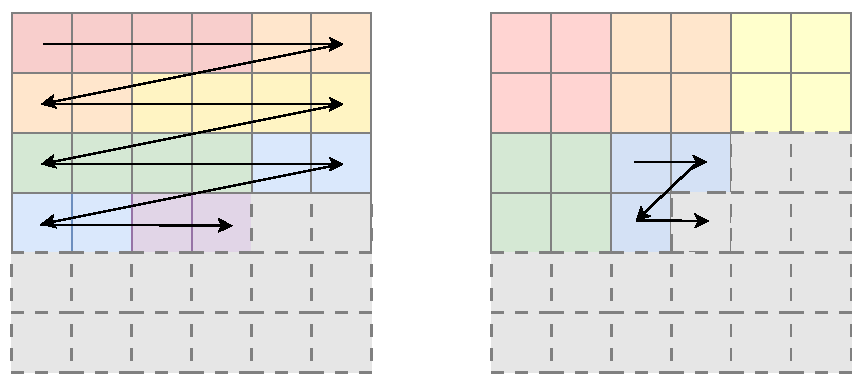
\includegraphics[width=0.6\linewidth]{figs/patchscan.drawio.pdf}
    \caption{Two ways to model 2D data sequentially. Left, raster scan, by taking bytes row by row and left to right; right, patch scan, where we first split an image into patches, and do raster scan across patches and within a patch. (T=36, K=9, P=4).
    }
    \label{fig:scan}
\end{figure}


\subsection{Patch scan vs Raster scan}

The patch scan method is inspired by recent works in Vision Transformers~\citep{vit}, and it is more effective than raster scan for modeling image sequencing. We found it improves both \megabyte and Perceiver AR. 
\begin{table}[h]
    \centering\small
    \begin{tabular}{ccccc}
    \toprule
 & (Global) Size & Local Size  & context  & bpb \\
    \midrule
\megabyte~(patch scan) & 62M (D=768, L=6) & N/A  & 8,192 (768 latents)  & 3.158                   \\
\megabyte~(raster scan) & 62M (D=768, L=6) & N/A  & 8,192 (768 latents)  & 3.428                   \\
Perceiver AR~(patch scan)  & 125M (D=768, L=12) & 125M (D=768, L=12) & 196,608 (patch size 192) & 3.373                   \\
Perceiver AR~(raster scan)  & 125M (D=768, L=12) & 125M (D=768, L=12) & 196,608 (patch size 192) & 3.552                  \\
    \bottomrule
    \end{tabular}
    \caption{ImageNet256 performance with patch scan vs raster scan for \megabyte and Perceiver AR.}
    \label{tab:patch_vs_raster}
\end{table}



\subsection{Longer sequence modeling}
\label{sec:long_text}
For our pg19 scaling experiment, we also use longer context length for \megabyte. The results are shown in Table~\ref{tab:longer_seq}. With longer sequence, we didn't observer further improvement, consistent with findings in ~\citet{perceiverar}. We think we will benefit more from longer sequence when we futher scale up the model size and data. 

\begin{table}[h]
    \centering
    \begin{tabular}{ccc}
    \toprule
 & context  & bpb \\
    \midrule
\megabyte &  8,192 (patch size 8)  & 0.8751                 \\
\megabyte &  16,384 (patch size 8)  & 0.8787                  \\
    \bottomrule
    \end{tabular}
    \caption{Longer sequence for PG19 dataset. For both experiments, we set global model as 1.3b, local model as 350m, and \megabyte patch size as 8.}
    \label{tab:longer_seq}
\end{table}




\end{document}


% This document was modified from the file originally made available by
% Pat Langley and Andrea Danyluk for ICML-2K. This version was created
% by Iain Murray in 2018, and modified by Alexandre Bouchard in
% 2019 and 2021 and by Csaba Szepesvari, Gang Niu and Sivan Sabato in 2022. 
% Previous contributors include Dan Roy, Lise Getoor and Tobias
% Scheffer, which was slightly modified from the 2010 version by
% Thorsten Joachims & Johannes Fuernkranz, slightly modified from the
% 2009 version by Kiri Wagstaff and Sam Roweis's 2008 version, which is
% slightly modified from Prasad Tadepalli's 2007 version which is a
% lightly changed version of the previous year's version by Andrew
% Moore, which was in turn edited from those of Kristian Kersting and
% Codrina Lauth. Alex Smola contributed to the algorithmic style files.
